\documentclass{beamer}
\usetheme{CambridgeUS}
%\usebeamercolor{lily}
\useoutertheme{infolines}
\usepackage{graphicx}
\usepackage{setspace}
\usepackage{tabularx}
\usepackage{tikzsymbols}
\usepackage{tikz}
\usepackage{spot}
\usepackage{tabularx}
\usepackage[absolute,overlay]{textpos}
\usepackage{booktabs}
\usepackage[backend=biber, style=authoryear]{biblatex}
%\addbibresource{biblio.bib}


\newcommand\Factor{1.2}

\AtBeginSection[]{
	\begin{frame}
		\setbeamercolor{coloredboxstuff}{fg=template, bg=template!20}
		\vfill
		\centering
		\begin{beamercolorbox}[sep=8pt,center,shadow=true,rounded=true]{coloredboxstuff}
			\large\textsc\insertsectionhead\par%
		\end{beamercolorbox}
		\vfill
	\end{frame}
}

\setbeamerfont{subtitle}{size=\large, series=\bfseries}
\definecolor{template}{RGB}{54, 114, 89}
\setbeamercolor{frametitle}{fg=template, bg=white}
\setbeamercolor{section in head/foot}{bg=template}
\setbeamercolor{subsection in head/foot}{bg=template!20, fg=template}
\setbeamercolor{author in head/foot}{bg=template}
\setbeamercolor{date in head/foot}{fg=template}
\setbeamercolor{title in head/foot}{fg=template}
\setbeamercolor{title}{fg=template}
\setbeamercolor*{item}{fg=template}
\setbeamertemplate{frametitle}[default][center]

\definecolor{back}{RGB}{247, 251, 255}
\definecolor{map}{RGB}{111, 172, 232}
\definecolor{childmap}{RGB}{161, 200, 240}
\definecolor{nodemap}{RGB}{141, 170, 199}
\definecolor{rasch}{rgb}{0.0, 0.33, 0.71}
\definecolor{log}{rgb}{0.0, 0.65, 0.58}
\definecolor{diff}{RGB}{33, 113, 181}
\definecolor{single}{RGB}{106, 81, 163}
\definecolor{comp}{RGB}{35, 99, 70}
\definecolor{inc}{RGB}{191, 13, 43}
\definecolor{highlight}{rgb}{0.45, 0.31, 0.59}
\definecolor{section}{RGB}{51,51,179}
\definecolor{typical}{RGB}{8, 69, 148}
\definecolor{model}{RGB}{74, 20, 134}
\definecolor{orangered2}{RGB}{238,64,0}
\definecolor{royalblue3}{RGB}{58,95,205}
\definecolor{springgreen}{RGB}{0,205,102}
\definecolor{magenta}{RGB}{255,0,255}


\setbeamertemplate{footnote}{%
	\parindent 1em\noindent%
	\raggedright
	\insertfootnotetext\par%
}

  \tikzset{
	invisible/.style={opacity=0},
	visible on/.style={alt={#1{}{invisible}}},
	alt/.code args={<#1>#2#3}{%
		\alt<#1>{\pgfkeysalso{#2}}{\pgfkeysalso{#3}} % \pgfkeysalso doesn't change the path
	},
	every overlay node/.style={
		%draw=black,fill=white,rounded corners,
		anchor=north west, inner sep=0pt,
	},
}

\def\tikzoverlay{%
	\tikz[remember picture, overlay]\node[every overlay node]
}%

\AtBeginSubsection[] % Do nothing for \subsection*
{
	\begin{frame}
		\vfill
		\centering
		\begin{beamercolorbox}[sep=8pt,center,shadow=true,rounded=true]{title}
			\bfseries\insertsubsectionhead\par%
		\end{beamercolorbox}
		\vfill
	\end{frame}
}

\title[Implicit assessment]{Implicit assessment in psychology: \\ Myths, doubts, and practical applications}

\date{June 9\textsuperscript{th}-10\textsuperscript{th} 2022}
\institute{University of Padova}
\author[Ottavia Epifania]{\texorpdfstring{Dr. Ottavia M. Epifania\newline\url{ottavia.epifania@unipd.it}}{Author}}

\begin{document}
	\tikzstyle{every picture}+=[remember picture]
	
	


\begin{frame}[plain]
    \maketitle
\end{frame}
\begin{frame}{Contents}
	\tableofcontents
\end{frame}

\section[Implicit assessment]{Implicit assessment: Definitions and evolution}

\begin{frame}
	\vskip0pt plus 1fill
	In Greenwald \& Banaji (1995), implicit attitudes are taken to be:
	
	\vspace{5mm}
	\begin{quote}
		Introspectively unidentified--or inaccurately identified--traces of past experience that mediate favorable or unfavorable feelings, thoughts, or actions toward social objects
	\end{quote}

\begin{center}
	\begin{large}
		IMPLICIT $=$ UNCONSCIOUS
	\end{large}
\end{center}

Implicit attitudes express themselves through \textbf{automatic associations} 

\vskip0pt plus 1filll

\color{template}\rule{0.30\linewidth}{0.5pt}\\
\color{black}
\footnotesize{Greenwald, A. G., \& Banaji, M. R. (1995) Implicit Social Cognition: Attitudes, Self-Esteem, and Stereotypes.\emph{ Psychological Review}, 102-1, doi: 10.1037/0033-295X.102.1.4}


\end{frame}

\begin{frame}{Automatic associations}
	\begin{center}
		
\includegraphics[width=.50\linewidth]{snakeFlower.png}
	\end{center}

\begin{itemize}
	\item Beyond one's control 
	\item Activated by triggering stimuli
	\item Not subject to introspection
	\item  Fast and almost immediate
\end{itemize}
	
	
\end{frame}

\begin{frame}{Automatic associations and the unconscious}
	Studying automatic associations $=$ studying implicit attitudes
	
	\vspace{5mm}
	\begin{center}
		
\includegraphics[width=.10\textheight]{down.png}
		
		\vspace{5mm}
		Access the unconscious and investigate it
	\end{center}

\pause

\centering

\includegraphics[width=.70\linewidth]{wrong.jpg}

\end{frame}

\begin{frame}
	\vskip0pt plus 1filll
	
	Fazio \& Olson (2003):
	
	\vspace{3mm}
	
	\begin{quote}
		Being fast is associating snakes with negative attributes does not imply that you are unaware of your negative attitudes towards snakes! 
	\end{quote}

	\vspace{3mm}

The only thing you are unaware of: Your attitudes are being assessed $\rightarrow$ something is indeed implicit

	\vspace{3mm}
Implicitly assessed constructs vs. unconscious constructs

\vskip0pt plus 1filll

\color{template}\rule{0.30\linewidth}{0.5pt}\\
\color{black}
\footnotesize{Fazio, R. H., \& Olson, M. A. (2003). Implicit measures in social cognition research: Their meaning
	and use. \emph{Annual Review of Psychology, 54}(1), 297–
	327. https://doi.org/10.1146/annurev.psych.54.101
	601.145225}

\end{frame}

\subsection*{Implicit $=$ indirect}


\begin{frame}
	
	\begin{center}
		From: 
		
		\vspace{5mm}
		Explicit = conscious Vs. Implicit = unconscious 
		
		\vspace{5mm}
		to:
		
		\vspace{5mm}
		Explicit = direct Vs. Implicit = indirect 
	\end{center}
	
	\vspace{5mm}
	Empirical meaning of implicit
\end{frame}

\begin{frame}
	\vskip0pt plus 1filll
	Banaji \& Greenwald (2013): 
	
	\vspace{5mm}
	\begin{quote}
		Theoretical definition of implicit as unconscious
	\end{quote}

\vspace{5mm}
Greenwald \& Banaji (2017), Greenwald \& Lai (2020): 

\vspace{5mm}
\begin{quote}
	Empirical definition of implicit as indirect
\end{quote}
\vskip0pt plus 1filll

\color{template}\rule{0.30\linewidth}{0.5pt}\\
\color{black}
\footnotesize{Banaji, M. R., \& Greenwald, A. G. (2013). \emph{Blindspot:
	Hidden biases of good people}. Delacorte Press,\\ 
Greenwald, A. G., \& Banaji, M. R. (2017). The
implicit revolution: Reconceiving the relation
between conscious and unconscious. \emph{American Psychologist, 72}(9), 861–871. https://doi.org/10.1037/
amp0000238\\
Greenwald, A. G., \& Lai, C. K. (2020). Implicit social
cognition. \emph{Annual Review of Psychology, 71}, 419–
445. https://doi.org/10.1146/annurev-psych-010419-
050837
}
\end{frame}

\begin{frame}{Why...?}
	\begin{itemize}
		\item Lack of evidence for supporting the unconsciousness
		\item Issues with construct validity 
		\item Theory uncommitted definition
	\end{itemize}
\end{frame}

\section[IAT]{The Implicit Association Test}

\begin{frame}{Implicit Association Test}

	\tikzoverlay (n1) at (8cm, 0.5cm){%
		\begin{minipage}{0.3\linewidth}
			\centering	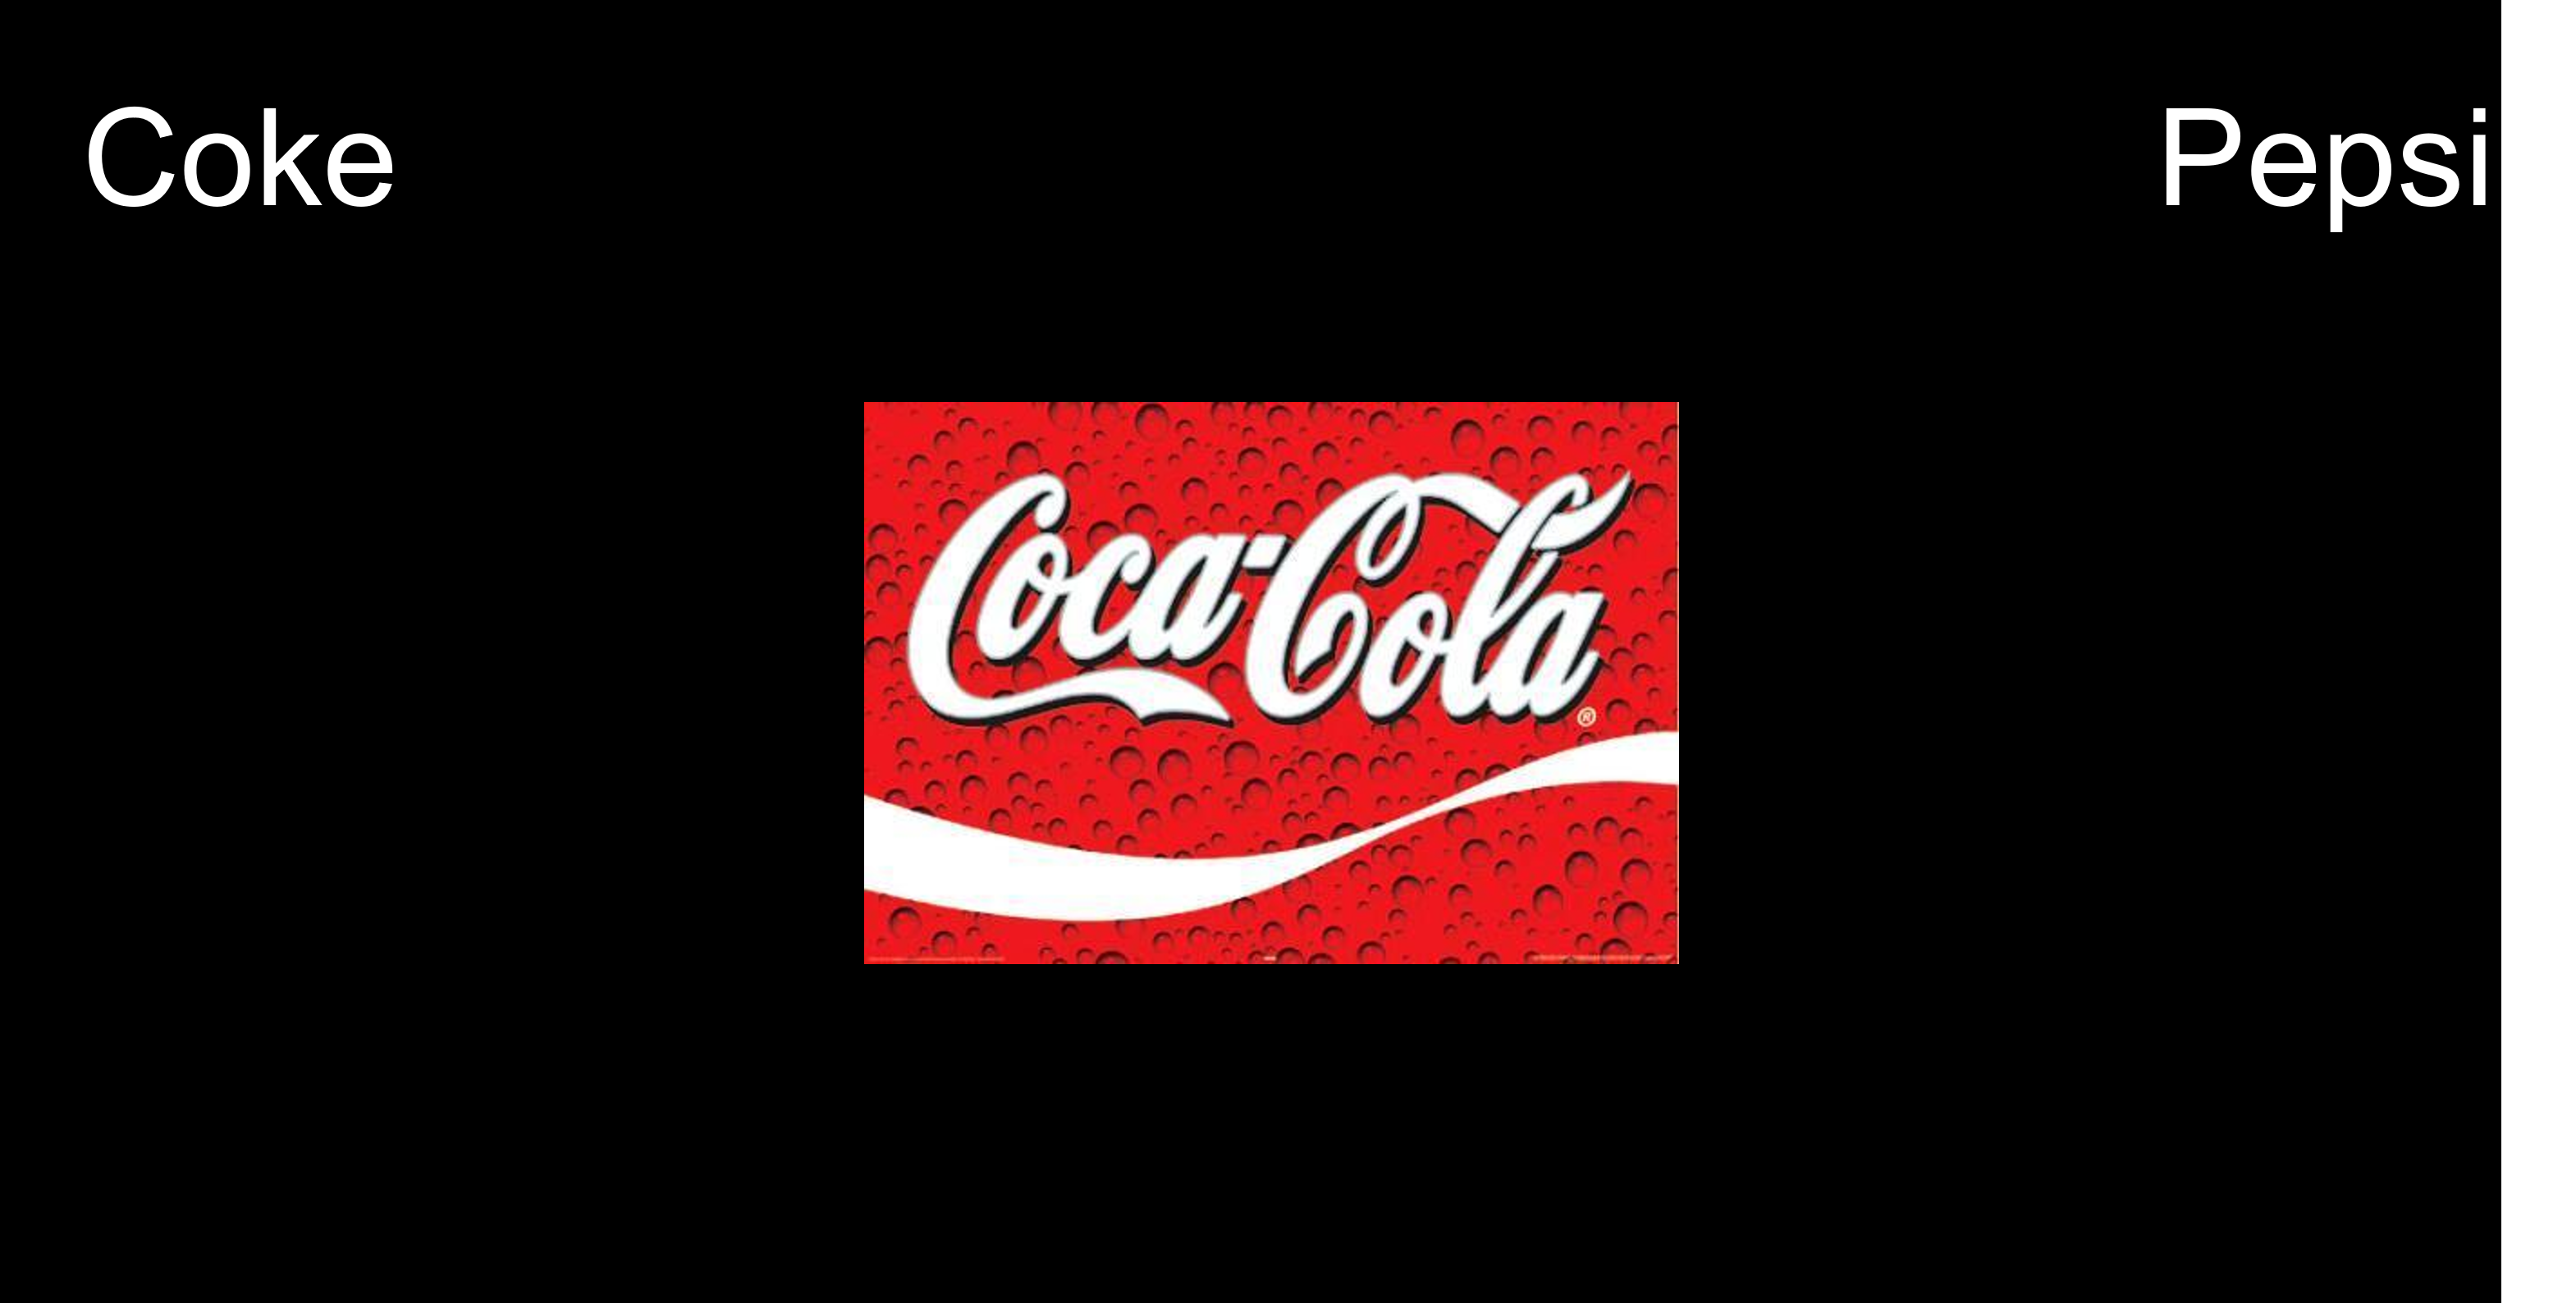
\includegraphics[width=\linewidth]{iatbase.png}
		\end{minipage}
	}; %

	Greenwald et al. (1998):
	
			\begin{spacing}\Factor
			\begin{table}
				\centering
				\caption{IAT}
				\begin{tabular}{c c c c }
					\hline
					Block	&	Trial	&	Left key	&	Right key	\\ \hline
					1	&	20	&	Good	&	Bad	\\
					2	&	20	&	Coke	&	Pepsi	\\
					\textcolor<2->{red}{3}	&	\textcolor<2->{red}{20}	&	\textcolor<2->{red}{Coke + Good}	&	\textcolor<2->{red}{Pepsi + Bad}	\\
					\textcolor<2->{red}{4}	&	\textcolor<2->{red}{40}	&	\textcolor<2->{red}{Coke + Good}	&	\textcolor<2->{red}{Pepsi + Bad}	\\
					5	&	20	&	Pepsi	&	Coke	\\
					\textcolor<3->{blue}{6}	&	\textcolor<3->{blue}{20}	&	\textcolor<3->{blue}{Pepsi + Good}	&	\textcolor<3->{blue}{Coke + Bad}	\\
					\textcolor<3->{blue}{7}	&	\textcolor<3->{blue}{40}	&	\textcolor<3->{blue}{Pepsi + Good}	&	\textcolor<3->{blue}{Coke + Bad}	\\
					\hline
				\end{tabular}
			\end{table}
		\end{spacing}

	


	\vspace{2mm}
\begin{columns}
	\begin{column}{.50\linewidth}
	\onslide<2-> \textcolor{red}{Coke-Good/Pepsi-Bad Condition}	
	\end{column}
\begin{column}{.50\linewidth}
	\onslide<3-> \textcolor{blue}{Pepsi-Bad/Coke-Good Condition}	
\end{column}

\end{columns}



%\color{template}\rule{0.30\linewidth}{0.5pt}\\
%\color{black}
%Greenwald, A. G., McGhee, D. E., \& Schwartz,
%	J. L. K. (1998). Measuring individual differences
%	in implicit cognition: The implicit association test.
%	Journal of Personality and Social Psychology,
%	74(6), 1464–1480. https://doi.org/10.1037/0022-
%	3514.74.6.1464
\end{frame}


\begin{frame}
	\begin{columns}
		\column{.5\linewidth}
		\centering{\textcolor{red}{Coke-Good/Pepsi-Bad (CGPB)}}
		\begin{figure}
			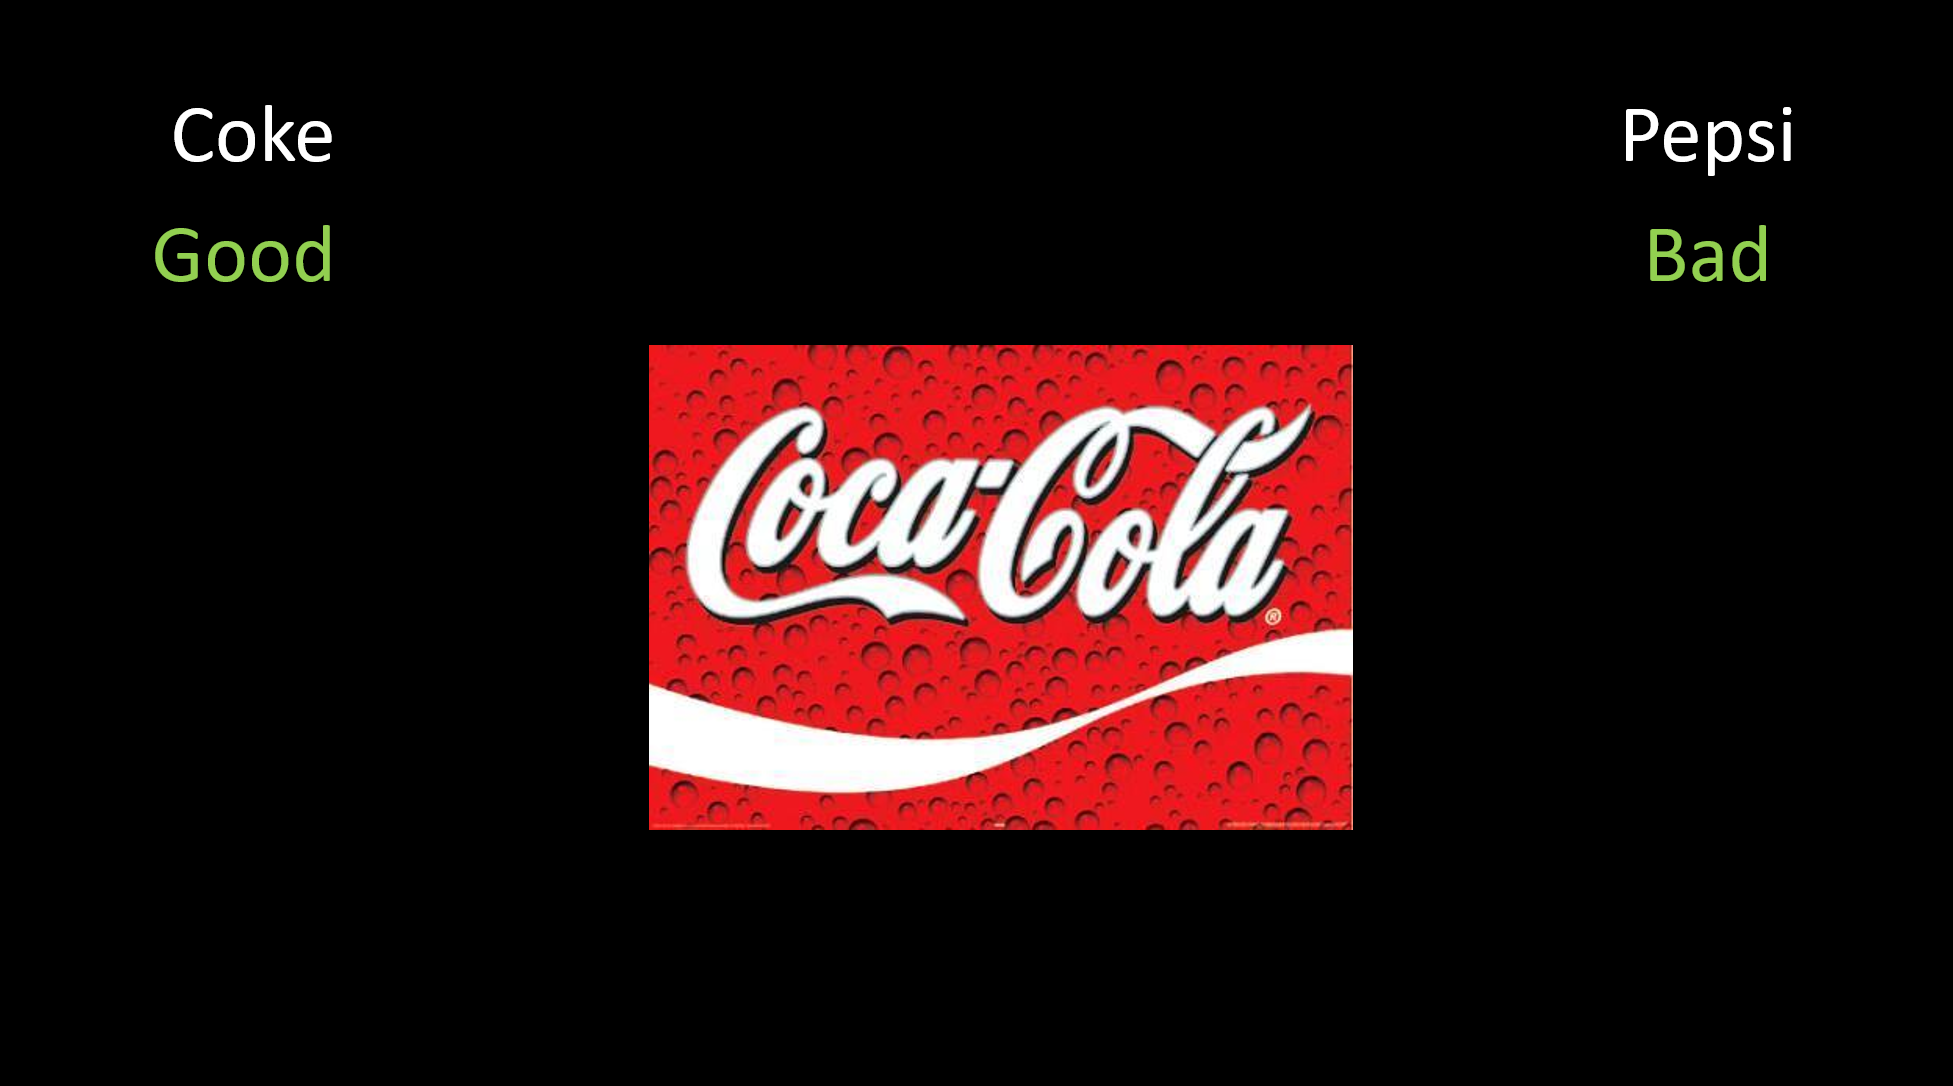
\includegraphics[width=\linewidth]{cocagood.png}
		\end{figure}
		
		\column{.5\linewidth}
		\centering{\textcolor{blue}{Pepsi-Good/Coke-Bad (PGCB)}}
		\begin{figure}
			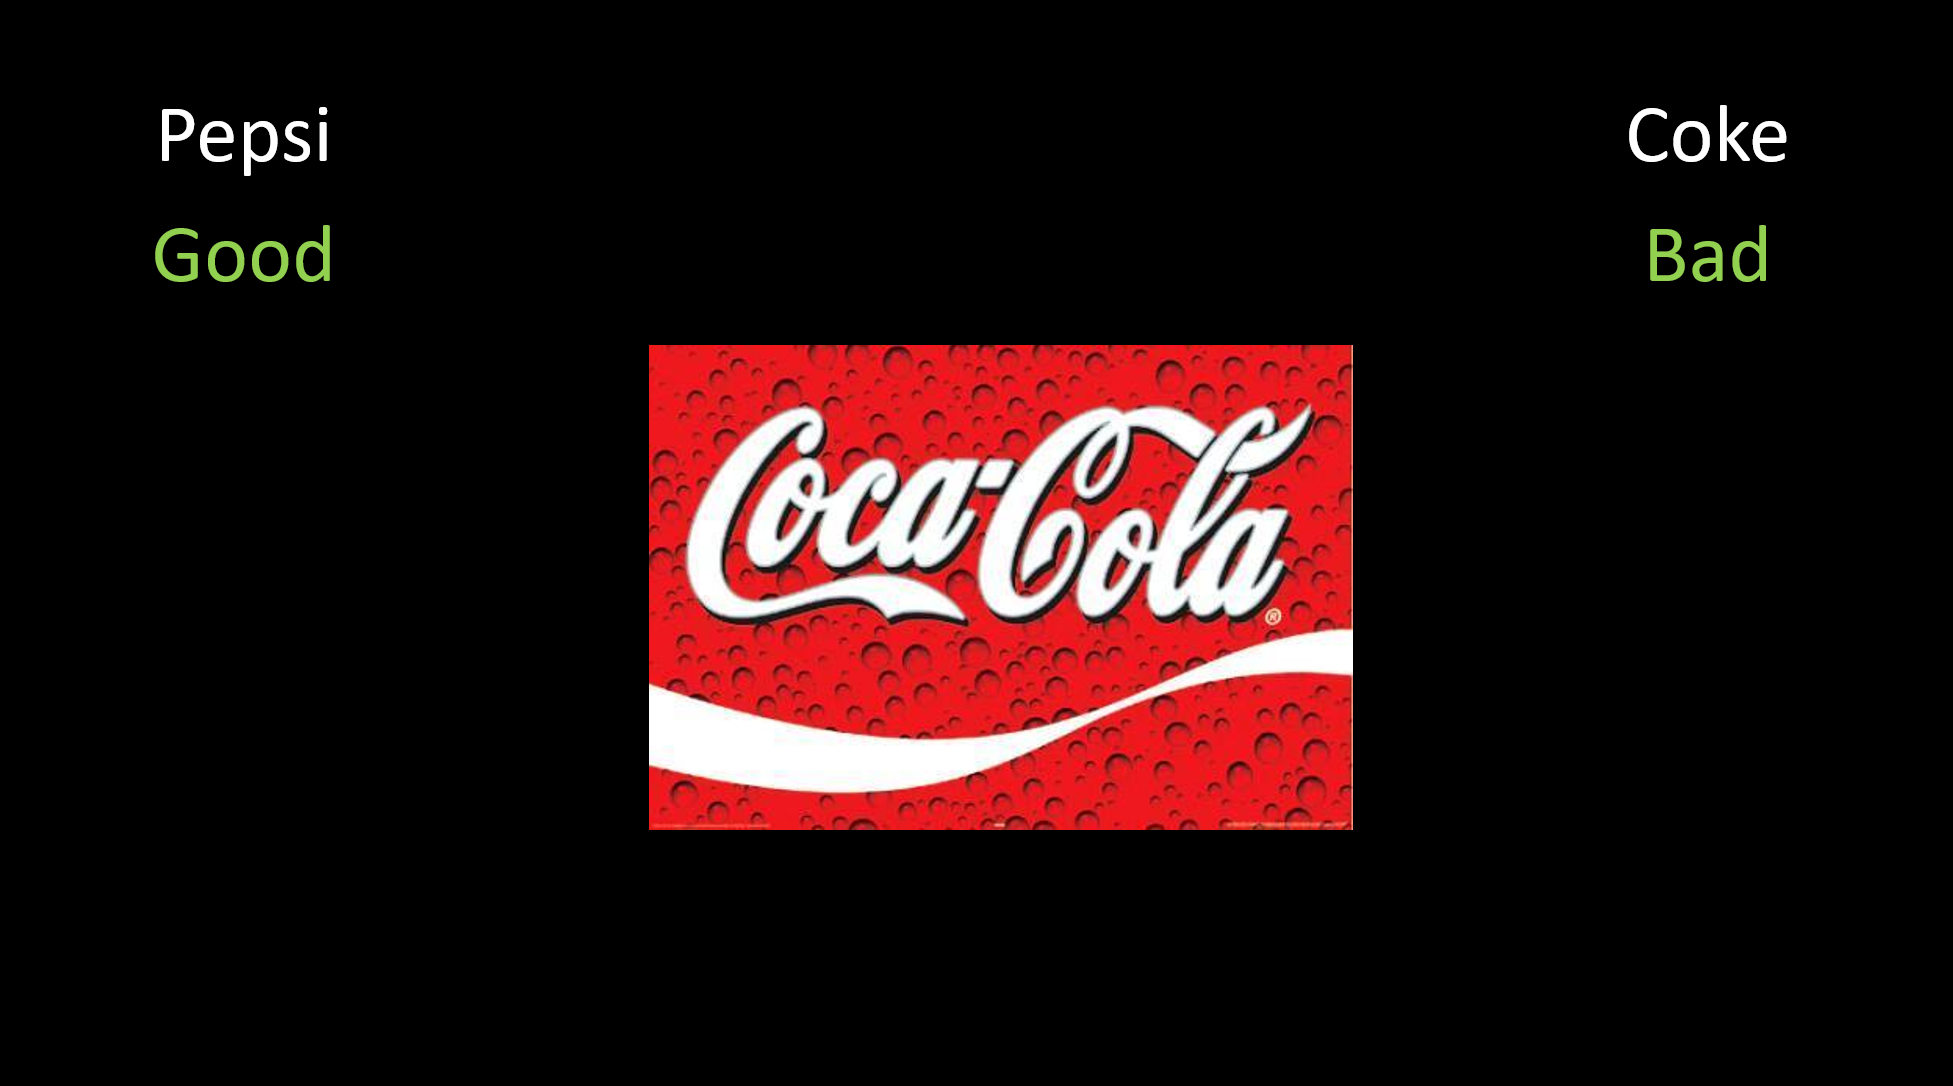
\includegraphics[width=\linewidth]{cocabad.png}
		\end{figure}
	\end{columns}

\end{frame}

\subsection*{Scoring}

\begin{frame}{\emph{D} score}
	\vskip0pt plus 1filll
Greenwald et al. (2003)
	
	\vspace{5mm}
	\begin{columns}
		\begin{column}{.50\linewidth}
			$$D_{\mathrm{B6,B3}} = \frac{M_{\mathrm{B6}} - M_{\mathrm{B4}}}{sd_{\mathrm{B6, B3}}}$$
		\end{column}
		\begin{column}{.50\linewidth}
			$$D_{\mathrm{B7,B4}} = \frac{M_{\mathrm{B7}} - M_{\mathrm{B4}}}{sd_{\mathrm{B7, B4}}}$$
	\end{column}
	\end{columns}
	
	\vspace{5mm}
		\begin{equation*}
		D = \frac{D_{\mathrm{B6,B3}} + D_{\mathrm{B7,B4}}}{2}
	\end{equation*}
	
	\vspace{5mm}
	Error responses? Fast responses?
	
	\vskip0pt plus 1filll
	
	\color{template}\rule{0.30\linewidth}{0.5pt}\\
	\color{black}
	\footnotesize{Greenwald, A. G., Nosek, B. A., \& Banaji, M. R.
		(2003). Understanding and using the implicit association test: I. An improved scoring algorithm. \emph{Journal
		of Personality and Social Psychology, 85}(2), 197–
		216. https://doi.org/10.1037/0022-3514.85.2.197}
\end{frame}

\begin{frame}
	
	\begin{spacing}\Factor
		\begin{table}[th!]
			\centering
			\caption{\label{tab:overview} Overview of the \emph{D} score algorithms.}
			\begin{tabularx}{\linewidth}{llll}
				\hline
				\emph{D score} & Error inflation & Lower tail treatment\\\hline
				\emph{D1} & Built-in correction & No \\
				\emph{D2} & Built-in correction & Delete trials $<$ 400 \emph{ms} \\
				\emph{D3} & Mean (correct responses) + 2\emph{sd} & No\\
				\emph{D4} & Mean (correct responses) + 600 \emph{ms} & No \\
				\emph{D5} & Mean (correct responses) + 2\emph{sd} & Delete trials $<$ 400 \emph{ms}\\
				\emph{D6} & Mean (correct responses) + 600 \emph{ms} & Delete trials $<$ 400 \emph{ms} \\\hline
			\end{tabularx}
		\end{table}
	\end{spacing}
\end{frame}

\section[What's wrong]{What's wrong with the IAT}
\vskip0pt plus 1filll

\begin{frame}{A measure in search of a construct}
	\begin{itemize}
		\item Lack of correlation with explicit measures
		\item Lack of correlation with actual behaviors
		\item Results are hard to reproduce
	\end{itemize}

\begin{center}
	YES BUT
\end{center}

\begin{itemize}
\item Correlation with explicit measures in socially non relevant topics
\item The type of behavior one tries to predict
\end{itemize}

\vskip0pt plus 1filll

\color{template}\rule{0.30\linewidth}{0.5pt}\\
\color{black}
\footnotesize{Carlsson, R., \& Agerstrom, J. (2016). A closer look at the discrimination outcomes in the IAT literature. \emph{Scandinavian Journal of Psychology, 57}(4), 278–287. doi:
	https://doi.org/10.1111/sjop.12288\\
Schimmack, U. (2021). The Implicit Association Test:
A method in search of a construct. \emph{Perspectives on
Psychological Science, 16}(2), 396–414. https://
doi.org/10.1177/1745691619863798}
\end{frame}

\begin{frame}{Laziness}
	\begin{itemize}
		\item What algorithm did you use? Don't know, don't care
		\item Error prone procedure
		\item Lack of automated and free software options
	\end{itemize}
\end{frame}

\begin{frame}{The \emph{D} score}
	\centering
		\begin{tabular}{l l l l l l l l}
		& \multicolumn{3}{c}{Condition A} & & \multicolumn{3}{c}{Condition B}\\
		Francesco & \Cat[2] & \Snowman[2] & \NiceReapey[2] & & \Cat[2] & \Snowman[2] & \NiceReapey[2] \\
		Giulia & \Cat[2] & \Snowman[2] & \NiceReapey[2] & & \Cat[2] & \Snowman[2] & \NiceReapey[2] \\
		Jessica & \Cat[2] & \Snowman[2] & \NiceReapey[2] & & \Cat[2] & \Snowman[2] & \NiceReapey[2] \\
	\end{tabular}
\end{frame}

\begin{frame}{However...}
	\begin{figure}
		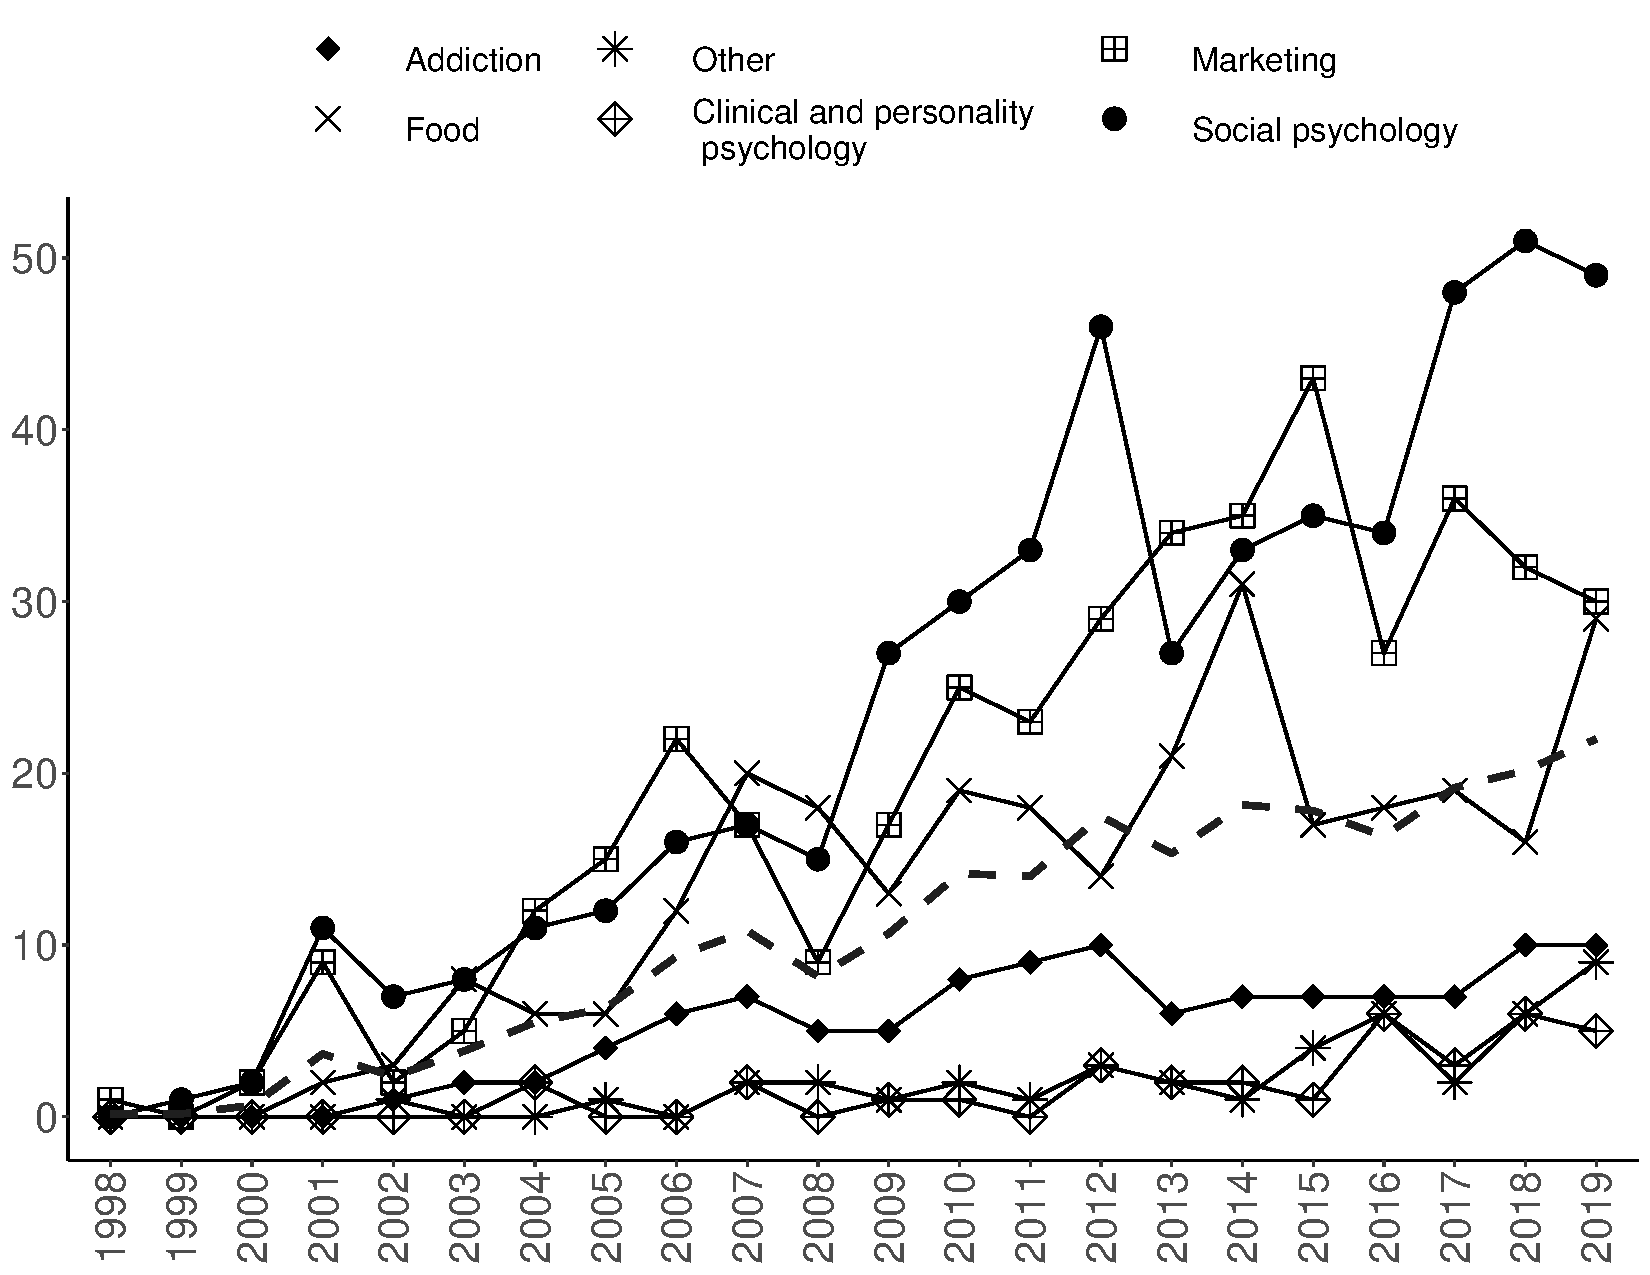
\includegraphics[width=.80\linewidth]{yearsIAT.pdf}
	\end{figure}
\end{frame}

\section[Not the only one]{One, not the only one}


\begin{frame}
	\onslide<1->
	\tikzoverlay (n1) at (1cm, 1cm){%
		\begin{minipage}{0.1\linewidth}
			\centering	
\includegraphics[width=\linewidth]{coca3.jpg}
		\end{minipage}
	}; %
	\onslide<1->
	\tikzoverlay (n2) at (7cm, 1cm){%
		\begin{minipage}{0.4\linewidth}
			\centering	
\includegraphics[width=0.25\linewidth]{pepsi3.jpg}
		\end{minipage}
	}; %
	\onslide<1->
	\tikzoverlay (n3) at (5cm, 0.5cm){%
		\begin{minipage}{0.4\linewidth}
			\huge \textbf{vs}
		\end{minipage}
	}; %	
	
	\onslide<2->
	
	\vspace{10mm}
	IAT $\rightarrow$ Comparative measure between contrasting objects:
	\vspace{5mm}
	\begin{itemize}
		\item The contrasted category is not always clear
		\vspace{5mm}
		\item The measure of the target category depends on the contrasted category
		\vspace{5mm}
		\item Maybe you want an ``absolute'' measure....
	\end{itemize}

\end{frame}

\begin{frame}{Single Category IAT}

\onslide<1->
\tikzoverlay (n1) at (1cm, 1cm){%
	\begin{minipage}{0.1\linewidth}
		\centering	
\includegraphics[width=\linewidth]{coca3.jpg}
	\end{minipage}
}; %


	Karpinski \& Steinman (2006):
		
	\begin{spacing}\Factor
		\begin{table}
				\centering
			\caption{SC-IAT}
			\begin{tabular}{c c c c}
				\hline
				Block	&	Trial	&	Left key	&	Right key	\\
				\hline
				1	&	24	&	Good + Coke	&	Bad	\\
				\textcolor<2->{red}{2}	&	\textcolor<2->{red}{72}	&	\textcolor<2->{red}{Good + Coke}	&	\textcolor<2->{red}{Bad}	\\
				3	&	24	&	Good 	&	Bad + Coke	\\
				\textcolor<3->{blue}{4}	&	\textcolor<3->{blue}{72}	&	\textcolor<3->{blue}{Good}	&	\textcolor<3->{blue}{Bad + Coke}	\\
				\hline
			\end{tabular}
		\end{table}
	\end{spacing}
	
	\begin{columns}
		\begin{column}{.50\linewidth}
			\centering
			\onslide<2->
			\textcolor{red}{Coke-Good condition}
		\end{column}
	
	\begin{column}{.50\linewidth}
		\onslide<3->
		\centering
		\textcolor{blue}{Coke-Bad condition}
	\end{column}
	\end{columns}

\vspace{5mm}
\onslide<4->
\begin{itemize}
	\item Response Time Window (rtw, usually 1,500 ms)
	\item Feedback to each response
\end{itemize}


\end{frame}

\subsection*{SC-IAT}
\begin{frame}{Scoring the SC-IAT}
	\vskip0pt plus 1filll
	\begin{equation*}
		Dscore = \frac{M_{\mathrm{B2}} - M_{\mathrm{B4}}}{s_{\mathrm{B2, B4}}}
	\end{equation*}

\vspace{5mm}

\begin{itemize}
	\item Responses $< 350$ms $ \rightarrow $ discarded
	\vspace{5mm}
	\item Responses $> rtw$ $ \rightarrow $ discarded
	\vspace{5mm}
	\item Error responses $\rightarrow$ $M + 400$ms 
\end{itemize}
\vskip0pt plus 1filll

\color{template}\rule{0.30\linewidth}{0.5pt}\\
\color{black}
\footnotesize{Karpinski, A., \& Steinman, R. B. (2006). The single
	category implicit association test as a measure of
	implicit social cognition.\emph{ Journal of Personality and
	Social Psychology, 91}(1), 16–32. https://doi.org/10
	.1037/0022-3514.91.1.16}

\end{frame}

\subsection*{GNAT}
\begin{frame}{Go/No-go association Task}
	Nosek \& Banaji (2001):
	
	\begin{footnotesize}
			\begin{spacing}\Factor
			\begin{table}
				\caption{GNAT}
				\begin{tabular}{c c c c }
					\hline
					Block	&	Trials	&	Signal	&	Noise	\\
					\hline
					1	&	16	&	Good	&	Bad	\\
					2	&	16	&	Bad	&	Good	\\
					3	&	16	&	Fruit	&	Bugs	\\
					4	&	16	&	Bugs	&	Fruit	\\
					\hline
					\textcolor<2>{blue}{5}	&	\textcolor<2>{blue}{16}	&	\textcolor<2>{blue}{Good + Fruit}	&	\textcolor<2>{blue}{Bad + Bugs}	\\
					&	\textcolor<2>{blue}{60}	&	\textcolor<2>{blue}{Good + Fruit}	&	\textcolor<2>{blue}{Bad + Bugs}	\\
					\textcolor<2>{red}{6}	&	\textcolor<2>{red}{16}	&	\textcolor<2>{red}{Bad + Fruit}	&	\textcolor<2>{red}{Good + Bugs}	\\
					&	\textcolor<2>{red}{60}	&	\textcolor<2>{red}{Bad + Fruit}	&	\textcolor<2>{red}{Good + Bugs}	\\
					\hline
					\textcolor<3>{blue}{7}	&	\textcolor<3>{blue}{16}	&	\textcolor<3>{blue}{Good + Bugs}	&	\textcolor<3>{blue}{Bad + Fruit}	\\
					&	\textcolor<3>{blue}{60}	&	\textcolor<3>{blue}{Good + Bugs}	&	\textcolor<3>{blue}{Bad + Fruit}	\\
					\textcolor<3>{red}{8}	&	\textcolor<3>{red}{16}	&	\textcolor<3>{red}{Bad + Bugs}	&	\textcolor<3>{red}{Good + Fruit}	\\
					&	\textcolor<3>{red}{60}	&	\textcolor<3>{red}{Bad + Bugs}	&	\textcolor<3>{red}{Good + Fruit}	\\
					\hline
				\end{tabular}
			\end{table}
		\end{spacing}
	\end{footnotesize}


\end{frame}



	\begin{frame}
		\vskip0pt plus 1filll
		
		\begin{columns}
			\column{.5\linewidth}
			\centering{\large{\textbf{\textcolor{green}{GO}}}}
			\begin{figure}
				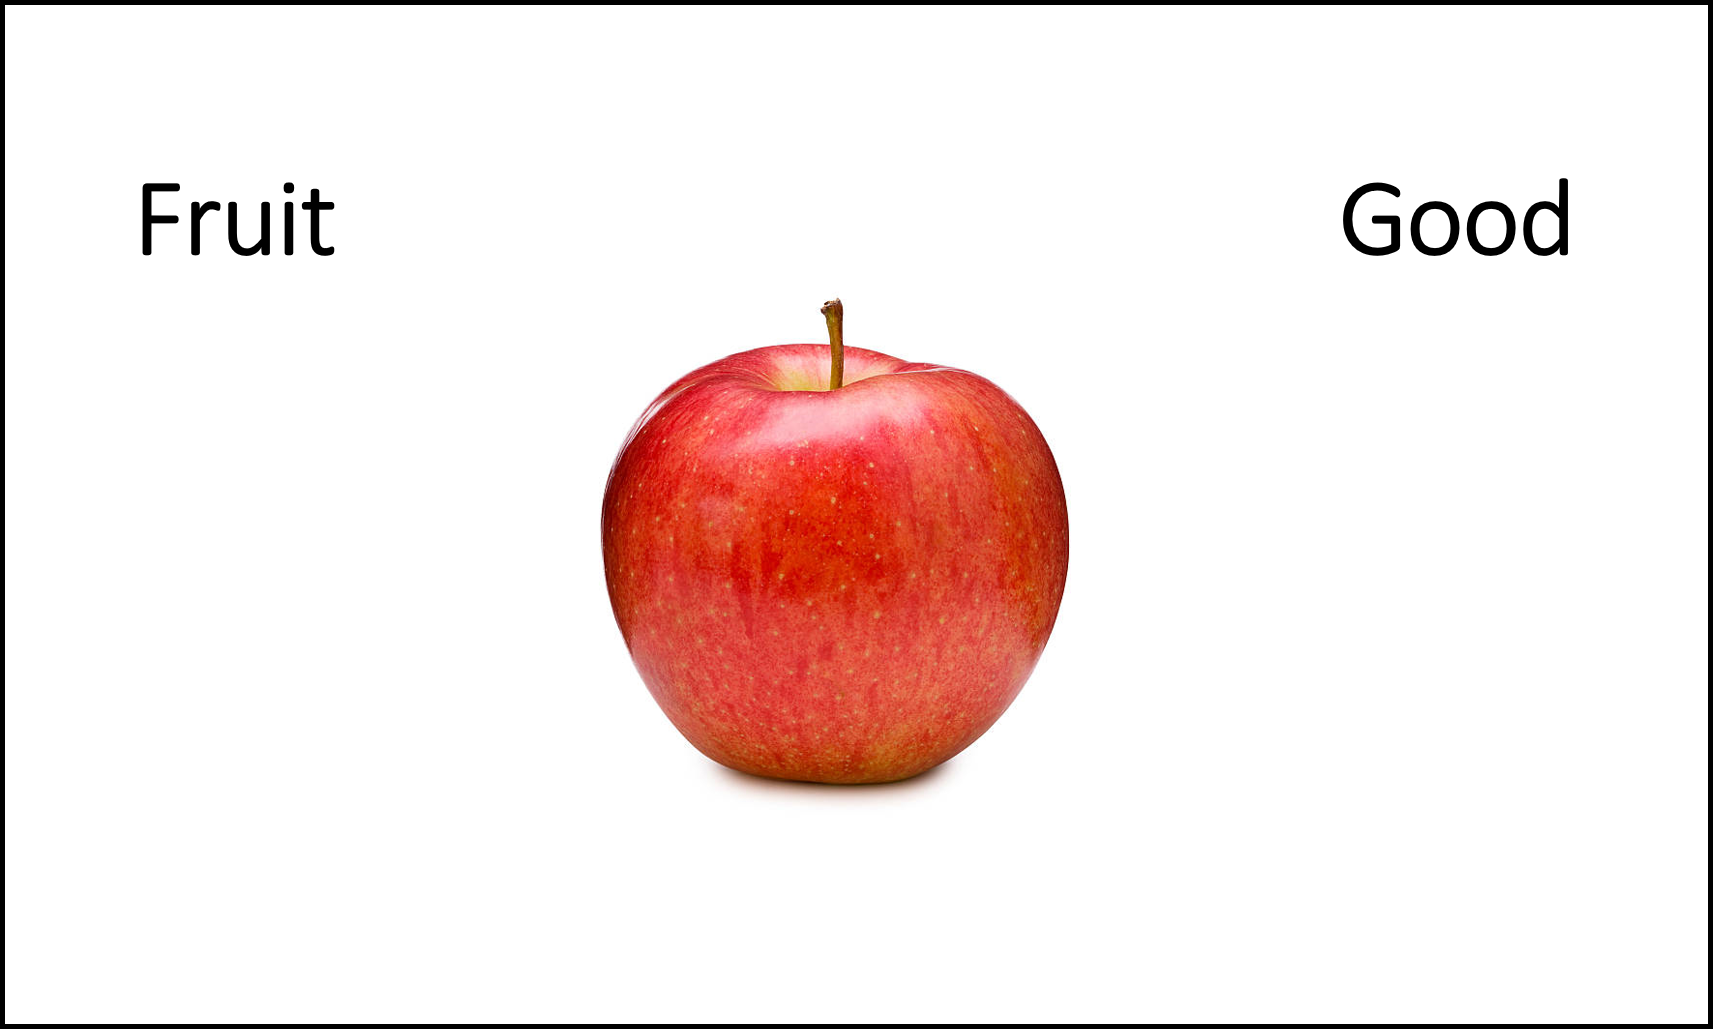
\includegraphics[width=\linewidth]{go.png}
			\end{figure}
			
			\column{.5\linewidth}
			\centering{\large{\textbf{\textcolor{red}{NO GO}}}}
			\begin{figure}
				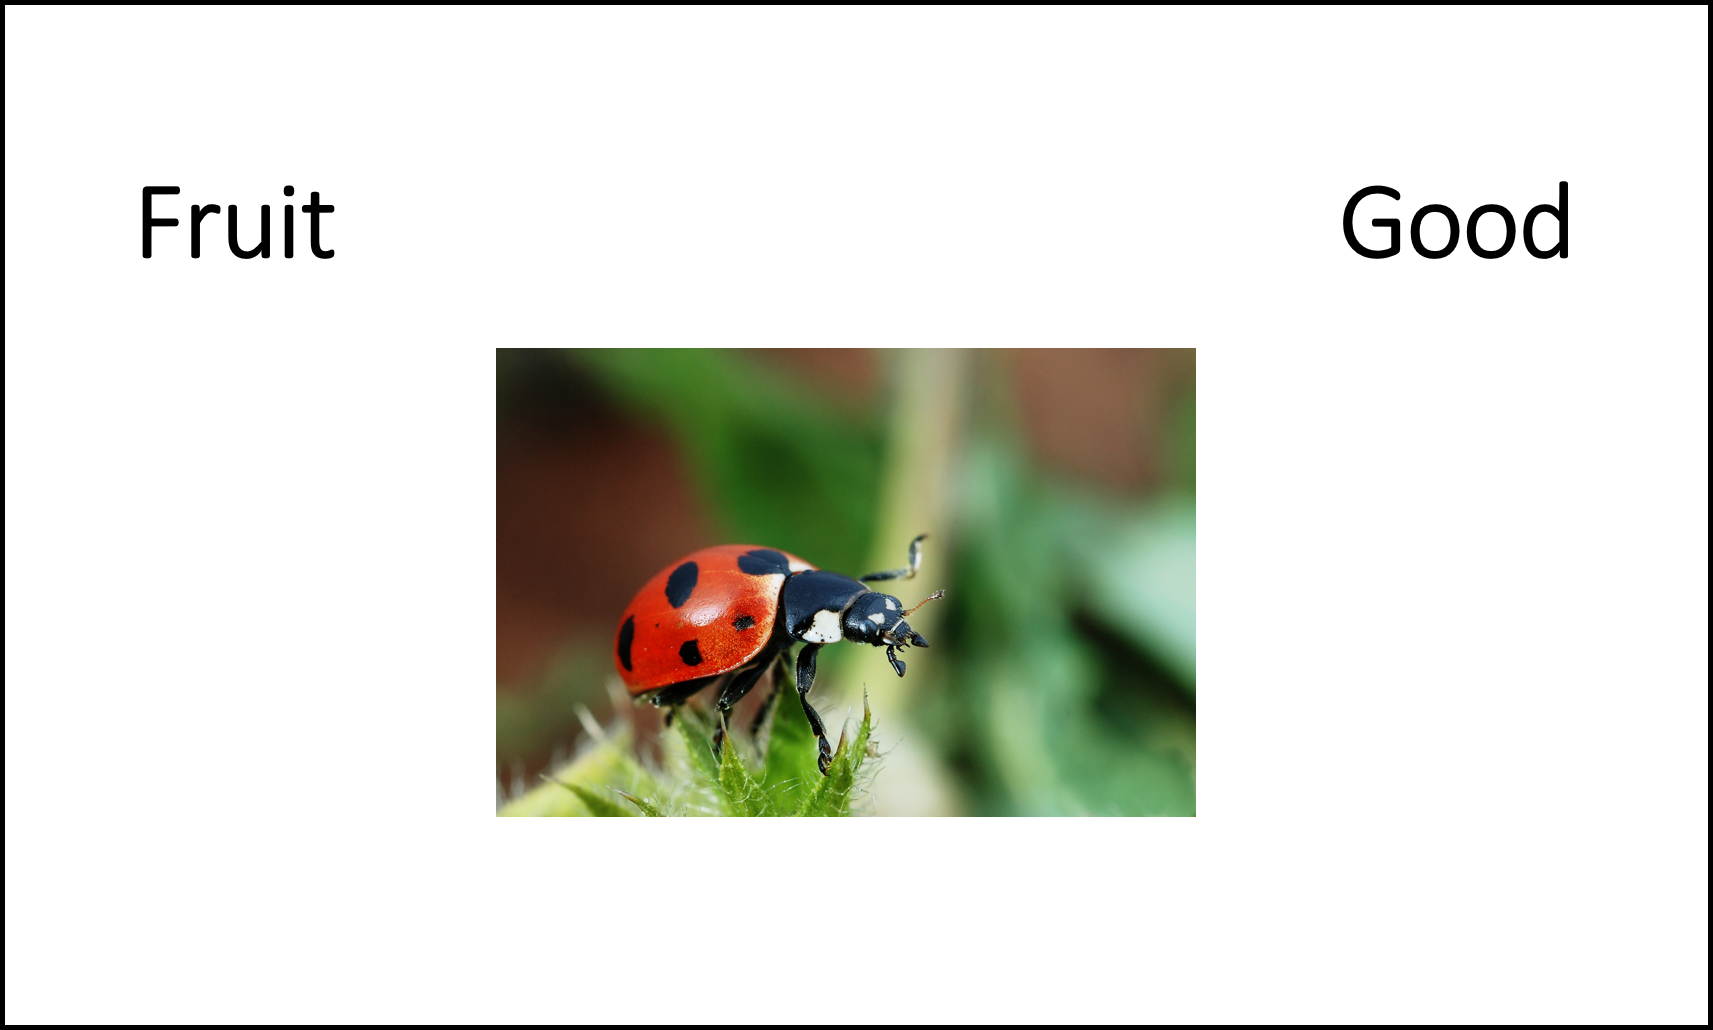
\includegraphics[width=\linewidth]{nogo.png}
			\end{figure}
		\end{columns}
	
	\vskip0pt plus 1filll
	
	
	\color{template}\rule{0.30\linewidth}{0.5pt}\\
	\color{black}
	
	\footnotesize{Nosek, B. A., \& Banaji, M. R. (2001). The go/no-go
		association task. \emph{Social Cognition, 19}(6), 625–666.
		Q21 https://doi.org/10.1521/soco.19.6.625.20886}
\end{frame}

\begin{frame}{Scoring}
	
$ d' $ (Green \& Swets, 1966): 

\vspace{5mm}

\begin{enumerate}
	\item $z$ score of the proportion of hits (correct ``go'' responses for signal items) 
	\item $z$ score of the proportion of false alarms (incorrect ``go'' responses for noise items)
	\item Difference between the two scores
\end{enumerate}
	
	\vspace{5mm}
	
	Empty cells (no false alarms or misses) $\rightarrow$ $0.35/\mathrm{number \, of \, trials}$
\end{frame}

\subsection*{Sorting Paired Features Task}
\begin{frame}{Sorting Paired Features Task}
	\vskip0pt plus 1filll
	Bar-Anan et. al (2009):
	
	\begin{footnotesize}
			\begin{spacing}\Factor
			\begin{table}
				\centering
				\caption{SPF}
				\begin{tabular}{c c c c c c}
					\hline
					Blocks	&	Trials	&	Top-left	&	Top-right	&	Bottom-left	&	Bottom-right	\\
					\hline
					1	&	48	&	Dogs+Good	&	Dogs+Bad	&	Cats+Good	&	Cats+Bad	\\
					2	&	48	&	Dogs+Bad	&	Dogs+Good	&	Cats+Bad	&	Cats+Good	\\
					3	&	48	&	Cats+Bad	&	Cats+Good	&	Dogs+Bad	&	Dogs+Good	\\
					4	&	48	&	Cats+Good	&	Cats+Bad	&	Dogs+Good	&	Dogs+Bad	\\
					\hline
					
				\end{tabular}
			\end{table}
		\end{spacing}
	\end{footnotesize}

\vspace{3mm}

To each pairing $ \rightarrow $ a response key

\vskip0pt plus 1filll

\color{template}\rule{0.30\linewidth}{0.5pt}\\
\color{black}
\footnotesize{Bar-Anan, Y., Nosek, B. A., \& Vianello, M. (2009).
	The sorting paired features task: A measure of
	association strengths. \emph{Experimental Psychology,
		56}(5), 329–343. https://doi.org/10.1027/1618-3169.
	56.5.329}
\end{frame}

\begin{frame}
			\begin{columns}
		\column{.5\linewidth}
		\centering{\large{Correct key: M}}
		\begin{figure}
			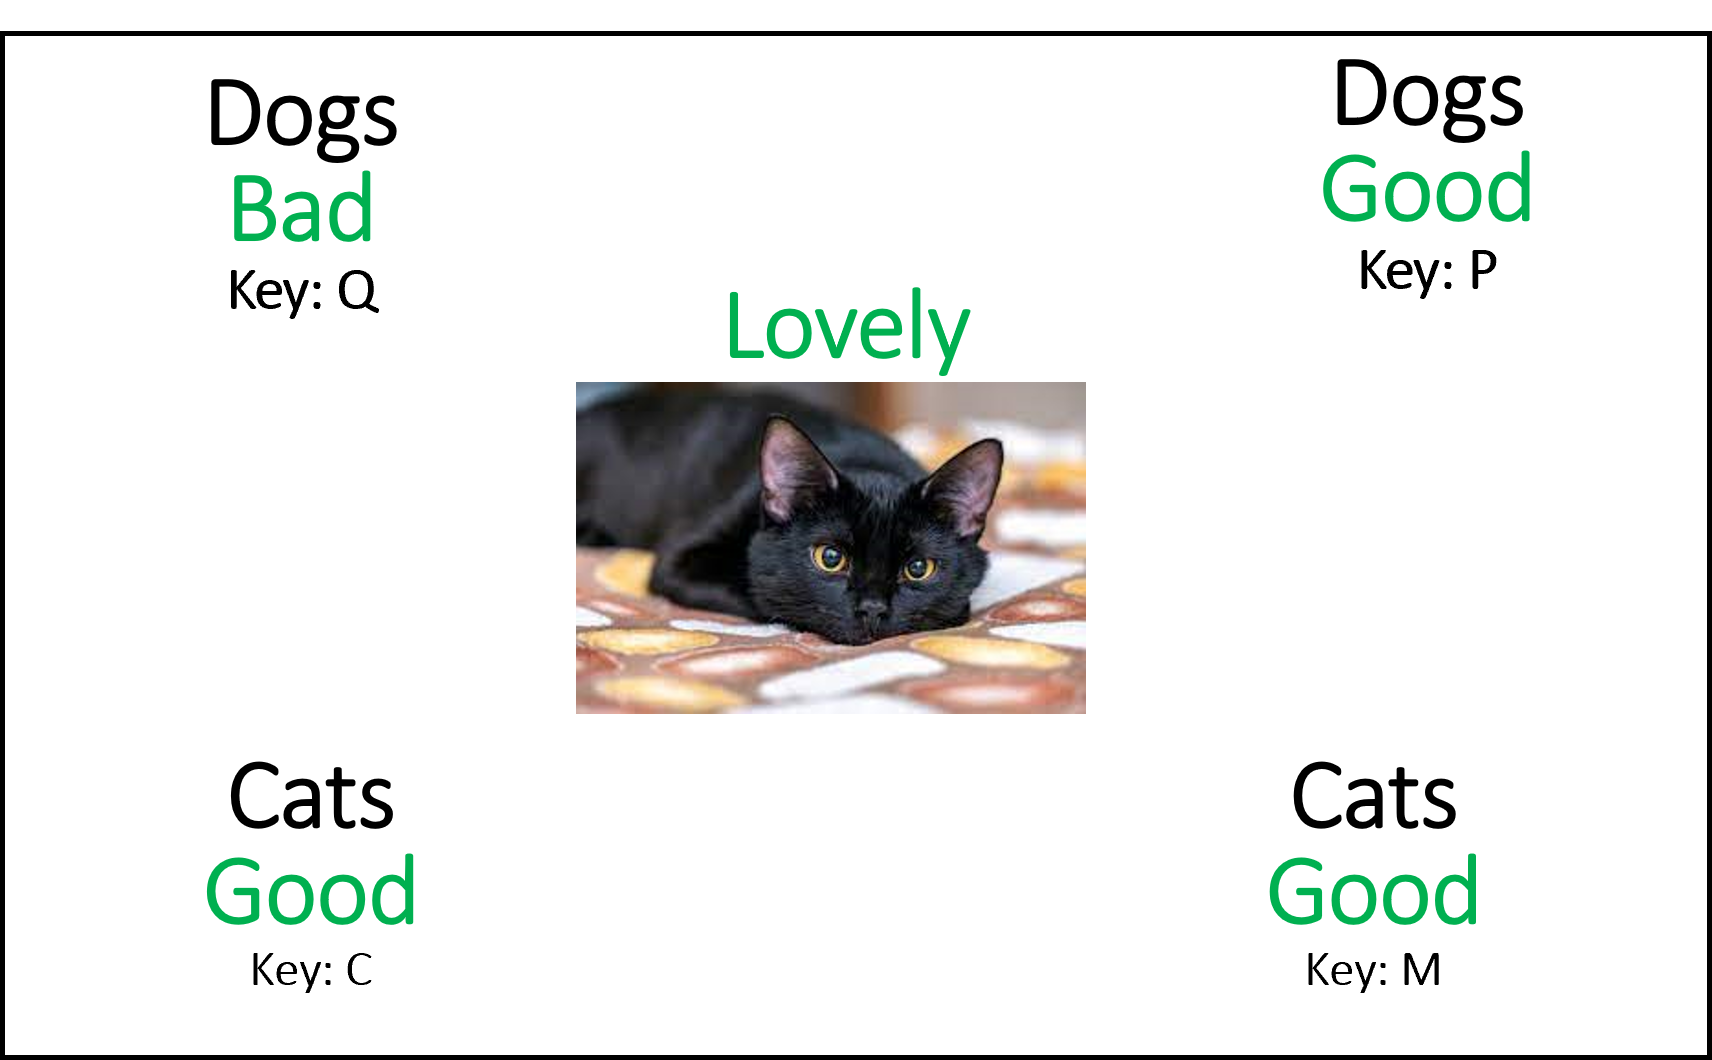
\includegraphics[width=\linewidth]{spf1.png}
		\end{figure}
		
		\column{.5\linewidth}
		\centering{\large{\large{Correct key: P}}}
		\begin{figure}
			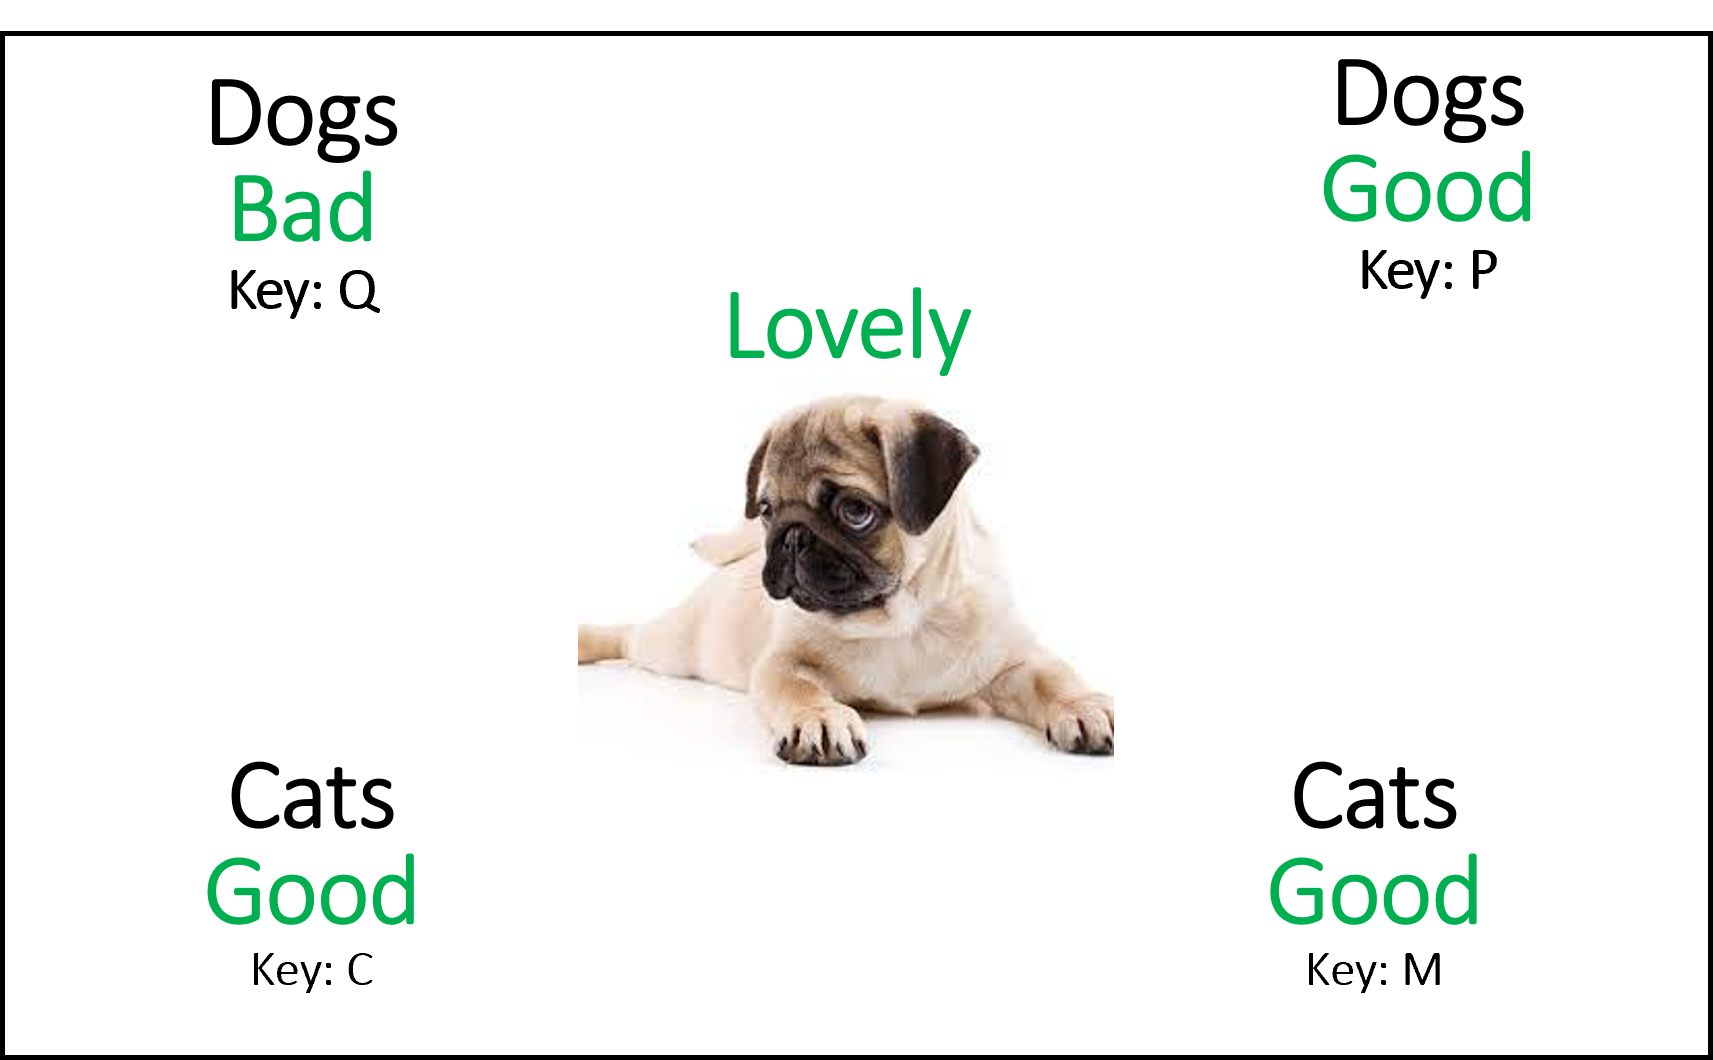
\includegraphics[width=\linewidth]{spf2.png}
		\end{figure}
	\end{columns}
\end{frame}

\section[Together]{Together is not always better}

\begin{frame}
	\tikzoverlay (n1) at (0cm,2.8cm){%
		\begin{minipage}{0.3\linewidth}
			\begin{center}
				\onslide<2->	\small{IAT} 
				
				\vspace{2mm}
				
				\onslide<1->
				
\includegraphics[width=0.3\linewidth]{coca3.jpg} VS 
\includegraphics[width=0.29\linewidth]{pepsi3.jpg}\end{center}
			
			\begin{block}
				
				
				\centering
				\includegraphics<2->[width=\linewidth]{cocagood.png}
			\end{block}
		\end{minipage}
	}; %	
	
	\tikzoverlay (n2) at (4cm, 3.3cm){%
		\begin{minipage}{0.3\linewidth}
			\begin{center}
				\onslide<2->
				\small{SC-IAT 1} 
				
				\onslide<1->
				\vspace{2mm}
				
\includegraphics[width=0.3\linewidth]{coca3.jpg} \end{center}
			\begin{block}
				
				\centering
				\includegraphics<2->[width=\linewidth]{sccokegood.png}
			\end{block}
		\end{minipage}
	}; %	
	
	\tikzoverlay (n3) at (8cm, 3.8cm){%
		\begin{minipage}{0.3\linewidth}
			\begin{center}
				\onslide<2->
				\small{SC-IAT 2}
				
				\onslide<1->
				\vspace{2mm}
				
\includegraphics[width=0.28\linewidth]{pepsi3.jpg}\end{center}
			
			\begin{block}
				
				\centering
				\includegraphics<2->[width=\linewidth]{scpepsigood.png}
			\end{block}
			
		\end{minipage}
	}; %
	\onslide<3->	
	\tikzoverlay (n4) at (-0.1cm, -2cm){%
		\begin{minipage}{0.3\linewidth}
			\begin{block}
				
				\centering
				\emph{D}  score
			\end{block}
		\end{minipage}
	}; %
	\tikzoverlay (n5) at (3.75cm, -2cm){%
		\begin{minipage}{0.3\linewidth}
			\begin{block}
				
				\centering
				\emph{D} Coke
			\end{block}
		\end{minipage}
	}; %
	\tikzoverlay (n6) at (7.6cm, -2cm){%
		\begin{minipage}{0.3\linewidth}
			\begin{block}
				
				\centering
				\emph{D} Pepsi
			\end{block}
		\end{minipage}
	}; %
	\onslide<3->
	\begin{tikzpicture}[remember picture, overlay]
		\path [line width=0.05cm,->,shorten >= +3pt, shorten <= +1pt] (n1.south) edge (n4.north);
		\path [line width=0.05cm,->,shorten >= +3pt, shorten <= +1pt] (n2.south)  edge (n5.north);
		\path [line width=0.05cm,->,shorten >= +3pt, shorten <= +1pt] (n3.south)  edge (n6.north);
	\end{tikzpicture}
\end{frame}


\begin{frame}
	
	%	\begin{itemize}
	
	\onslide<1-> 		
	
	\tikzoverlay (n0) at (-0cm,2.7cm) {%
		
		
		Stand alone measure:
		
	};%
	
	%	\item 
	\onslide <2->
	\tikzoverlay (n1) at (0.5cm,2.5cm) {%
		
		\centering	
		\begin{tabular}{l l l l l l l l}
			& \multicolumn{3}{c}{Condition A} & & \multicolumn{3}{c}{Condition B}\\
			Lara & \Cat[2] & \Snowman[2] & \NiceReapey[2] & & \Cat[2] & \Snowman[2] & \NiceReapey[2] \\
			Francesco & \Cat[2] & \Snowman[2] & \NiceReapey[2] & & \Cat[2] & \Snowman[2] & \NiceReapey[2] \\
			Giulia & \Cat[2] & \Snowman[2] & \NiceReapey[2] & & \Cat[2] & \Snowman[2] & \NiceReapey[2] \\
		\end{tabular}
		
	};%
	\\
	\onslide<1-> 
	
	\tikzoverlay (n5) at (-0cm,-0.2cm) {%
		
		Multiple measures: 
		
	};%
	
	
	
	
	\onslide<3->
	\tikzoverlay (n2) at (-0.6cm,-0.5cm) {%
		%	\begin{minipage}{0.8\textwidth}%
		
		\begin{tiny}
			
			\begin{tabular}{p{0.01cm} p{0.2cm} p{0.2cm} p{0.02cm} p{0.2cm} p{0.2cm} p{0.2cm}}
				\multicolumn{7}{c}{IAT} \\
				& \multicolumn{3}{c}{Condition A} &  \multicolumn{3}{c}{Condition B}\\
				L& \Cat[2] & \Snowman[2] & \NiceReapey[2] & \Cat[2] & \Snowman[2] & \NiceReapey[2] \\
				F & \Cat[2] & \Snowman[2] & \NiceReapey[2] & \Cat[2] & \Snowman[2] & \NiceReapey[2] \\
				G & \Cat[2] & \Snowman[2] & \NiceReapey[2] &  \Cat[2] & \Snowman[2] & \NiceReapey[2] \\
			\end{tabular}
		\end{tiny}
		
		%	\end{minipage}
	};%
	\tikzoverlay (n3) at (3.6cm,-0.5cm) {%
		%	\begin{minipage}{0.8\textwidth}%
		\begin{tiny}
			
			\begin{tabular}{p{0.01cm} p{0.2cm} p{0.2cm} p{0.02cm} p{0.2cm} p{0.2cm} p{0.2cm}}
				\multicolumn{7}{c}{SC-IAT 1} \\
				& \multicolumn{3}{c}{Condition A} &  \multicolumn{3}{c}{Condition B}\\
				L& \Cat[2] & \Snowman[2] & \NiceReapey[2] & \Cat[2] & \Snowman[2] & \NiceReapey[2] \\
				F & \Cat[2] & \Snowman[2] & \NiceReapey[2] & \Cat[2] & \Snowman[2] & \NiceReapey[2] \\
				G & \Cat[2] & \Snowman[2] & \NiceReapey[2] &  \Cat[2] & \Snowman[2] & \NiceReapey[2] \\
			\end{tabular}
		\end{tiny}
		
		%	\end{minipage}
	};%
	\tikzoverlay (n4) at (7.7cm,-0.5cm) {%
		%	\begin{minipage}{0.8\textwidth}%
		\begin{tiny}
			
			\begin{tabular}{p{0.01cm} p{0.2cm} p{0.2cm} p{0.02cm} p{0.2cm} p{0.2cm} p{0.2cm}}
				\multicolumn{7}{c}{SC-IAT 2} \\
				& \multicolumn{3}{c}{Condition A} &  \multicolumn{3}{c}{Condition B}\\
				L& \Cat[2] & \Snowman[2] & \NiceReapey[2] & \Cat[2] & \Snowman[2] & \NiceReapey[2] \\
				F & \Cat[2] & \Snowman[2] & \NiceReapey[2] & \Cat[2] & \Snowman[2] & \NiceReapey[2] \\
				G & \Cat[2] & \Snowman[2] & \NiceReapey[2] &  \Cat[2] & \Snowman[2] & \NiceReapey[2] \\
			\end{tabular}
		\end{tiny}
		
		%	\end{minipage}
	};%
	
	\onslide<3->
	\begin{tikzpicture}[remember picture, overlay]
		\path [<->] (n2) edge[bend right=50] (n3);
		\path [<->] (n3) edge[bend right=50] (n4);
		\path [<->] (n2) edge[bend right=50] (n4);
		
	\end{tikzpicture}
	
\end{frame}

\section[The workaround]{A possible workaround}

\begin{frame}{The supermodel(s)}
	\vskip0pt plus 1filll
	\begin{center}
		\Large{\textbf{Linear Mixed-Effects Models}} (LMMs)
	\end{center}
	
	\vspace{5mm}
	\begin{itemize}
		\item[{\small
\includegraphics[height=3ex]{supergirl.png}}] Account for (potentially) all the sources of variability and dependency
		\vspace{1.5mm}
		\item[{\small
\includegraphics[height=3ex]{supergirl.png}}] Gather information at the stimulus level
		\vspace{1.5mm}
		\item[{\small
\includegraphics[height=3ex]{supergirl.png}}] Estimate the Rasch and log-normal models 
	\end{itemize}

\vskip0pt plus 1filll

\color{template}\rule{0.30\linewidth}{0.5pt}\\
\color{black}
\footnotesize{Epifania, O. M., Robusto, E., \& Anselmi, P. (2021). Rasch gone mixed: A mixed model approach to
	the Implicit Association Test. \emph{Testing, Psychometrics, Methodology in Applied Psychology,
	28}, 467–483. doi: 10.4473/TPM28.4.5}
\end{frame}

\begin{frame}{From Linear to Rasch and log-normal}
	
	\begin{figure}
		\begin{overprint}
			\onslide<1>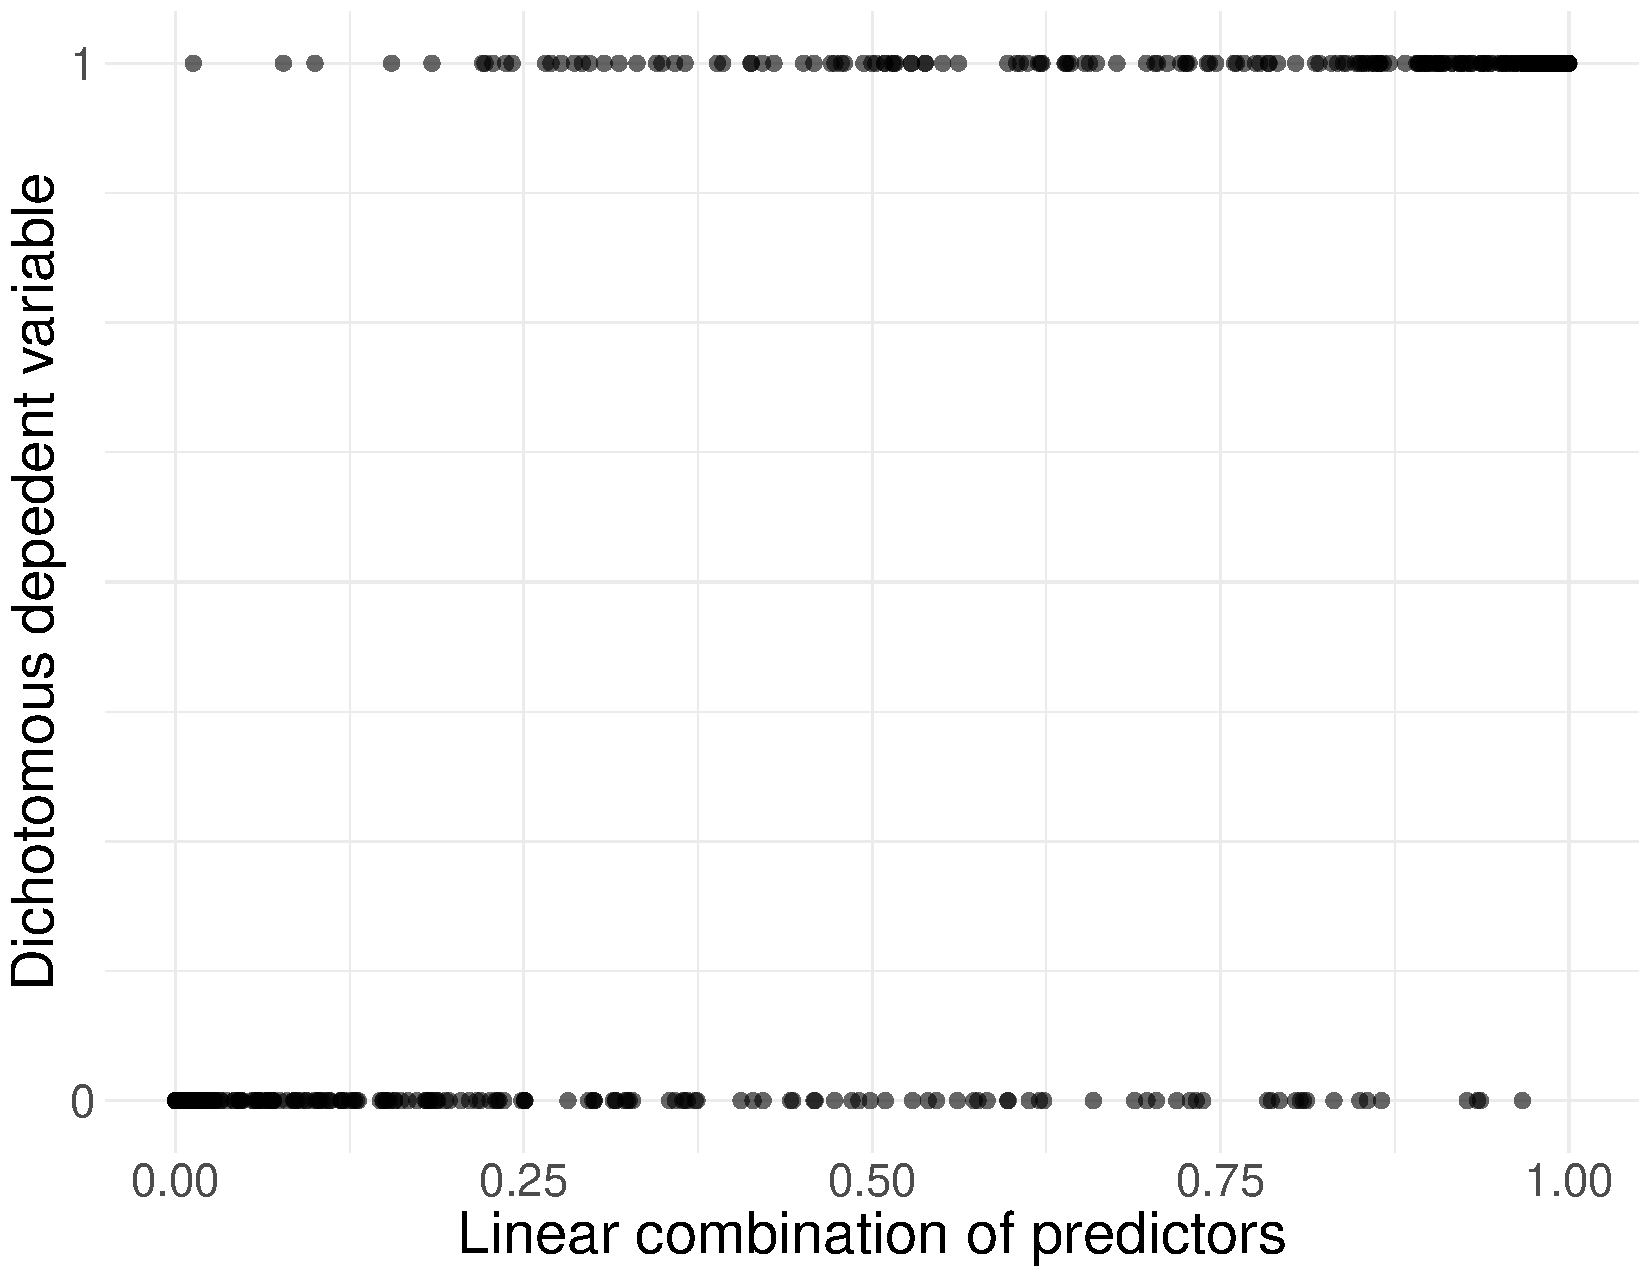
\includegraphics[width=0.7\linewidth]{baseGLM.pdf}
			\onslide<2>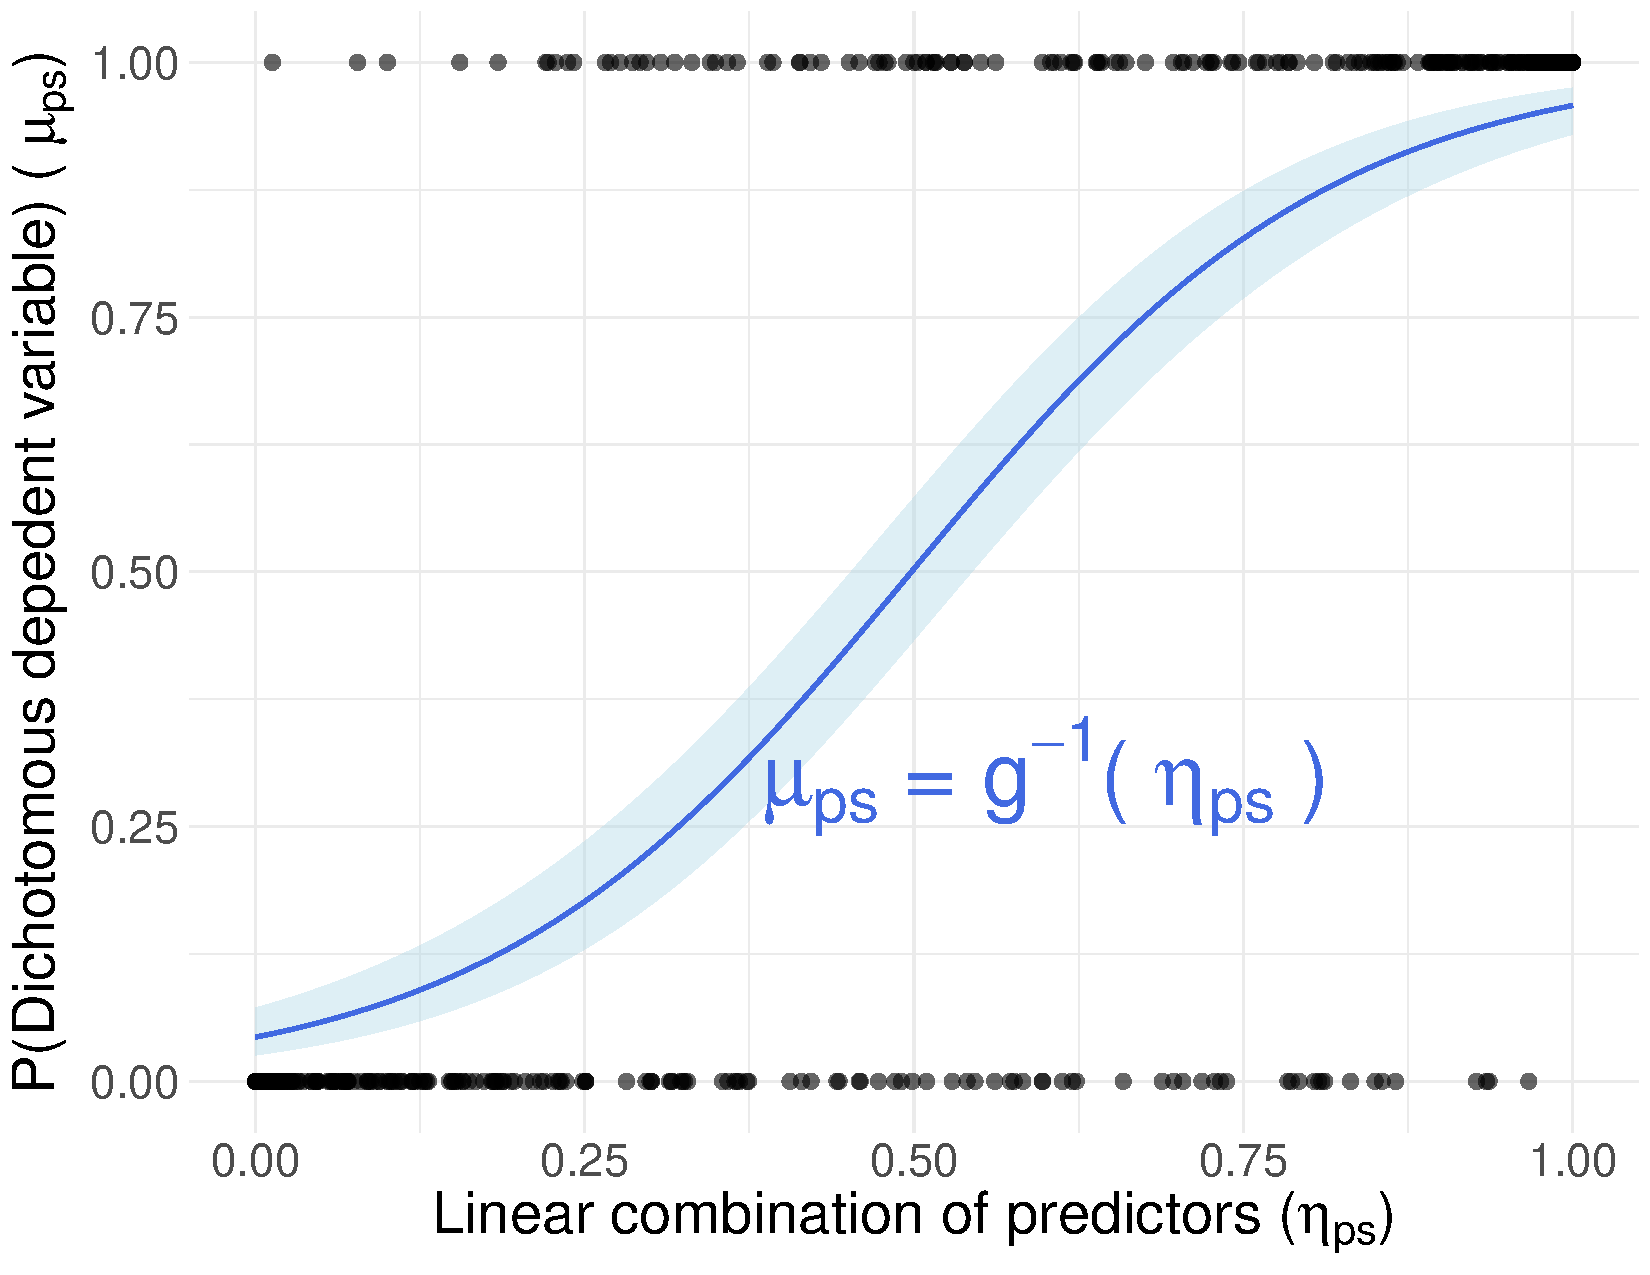
\includegraphics[width=0.7\linewidth]{linkGLM.pdf}
		\end{overprint}
	\end{figure}
	
	\onslide<2->
	\tikzoverlay (n1) at (8cm, 5.6cm){%
		\begin{minipage}{0.7\linewidth}
			
			\emph{Logit link function g}
			
			$g(\eta_{ps}) = log\left(\frac{\mu_{ps}}{1 - \mu_{ps}}\right)$
			
			\vspace{5mm}
			
			\emph{Inverse} $g^{-1}$
			
			\vspace{5mm}
			
			$g^{-1} = \frac{exp(\eta_{ps})}{1 + exp(\eta_{ps})} $
			
			\vspace{1.5mm}
			where $\eta_{ps} = \theta_p + b_s$
		\end{minipage}
	}; 
	
\end{frame}

\begin{frame}
	
	
	
	\begin{columns}[T] % align columns
		\begin{column}{.50\linewidth}
			\textcolor{diff}{\rule{\linewidth}{2pt}}
			\begin{center}
				\textcolor{diff}{	\large{{Standard}}}
			\end{center}
			
		\end{column}
		
		\hfill%
		\begin{column}{.50\linewidth}
			\textcolor{single}{\rule{\linewidth}{2pt}}
			\begin{center}
				\textcolor{single}{\large{{(G)LM}}}	
			\end{center}
			
		\end{column}%
	\end{columns}
	
	\vspace{1.5mm}
	
	\begin{center}
		\Large\textcolor{rasch}{Rasch model}
	\end{center}
	
	\begin{columns}[T]
		\begin{column}{.50\linewidth}
			\vspace{1.5mm}
			$P(x_{ps} = 1) = \displaystyle \frac{exp(\theta_p \spot<2-2>[fill=rasch!50]{-} b_s)}{1 + exp(\theta_p \spot<2-2>[fill=rasch!50]{-} b_s)}$
		\end{column}
		\hfill
		
		\begin{column}{.50\linewidth}
			
			
			\vspace{1.5mm}
			$P(x_{ps} = 1) = \displaystyle \frac{exp(\theta_p \, \spot<2-2>[fill=rasch!50]{+} \, b_s)}{1 + exp(\theta_p \, \spot<2-2>[fill=rasch!50]{+} \, b_s)}$
		\end{column}
	\end{columns}
	
	
	\vspace{5mm}
	\begin{center}
		\Large\textcolor{log}{Log-normal model}
	\end{center}
	
	
	\begin{columns}[T]
		\begin{column}{.50\linewidth}
			\centering
			$f (t_{ps}) =  \delta_s \, \spot<2-2>[fill=log!50]{-} \, \tau_p \, + \, \varepsilon $
		\end{column}
		\hfill
		
		\begin{column}{.50\linewidth}
			\centering
			$f(t_{ps}) =  \delta_s \, \spot<2-2>[fill=log!50]{+} \, \tau_p \, +  \, \varepsilon$
		\end{column}
	\end{columns}	
\end{frame}

\begin{frame}
	\begin{footnotesize}
		The expected response $y$ for the observation $i = 1, \ldots, I$ for respondent $p = 1,\ldots, P$ on stimulus $s = 1,\ldots, S$ in condition $c= 1,\ldots, C$:
	\end{footnotesize}
	\footnotesize
	
	\vspace{3mm}
	Model 1:
	\begin{equation*}\label{AccuracyMin}
		y_{i} = \spot[fill =blue!15]{\alpha + \beta_c X_c}  + \spot[fill=yellow!20]{\alpha_{p[i]} +  \alpha_{s[i]} + \varepsilon_{i}}
	\end{equation*}
	\begin{centering}
		
		$\alpha_p \sim \mathcal{N}(0, \sigma_p^2)$,
		
	\end{centering}
	
	\begin{centering}
		
		$\alpha_s \sim \mathcal{N}(0, \sigma_s^2)$.
		
	\end{centering}
	
	
	
	Model 2: 
	\begin{equation*}\label{Accuracy5}
		y_{i} = \spot[fill =blue!15]{\alpha + \beta_c X_c}  + \spot[fill=yellow!20]{ \alpha_{p[i]} +  \beta_{s[i]}c_{i} + \varepsilon_{i}}
	\end{equation*}
	
	\begin{centering}
		$\alpha_p \sim \mathcal{N}(0, \sigma_p^2)$,
		
	\end{centering}
	
	\begin{centering}
		
		$\beta_s \sim \mathcal{MVN}(0, \Sigma_{sc})$.
		
	\end{centering}
	
	Model 3: 
	
	\begin{equation*}
		y_{i} = \spot[fill =blue!15]{\alpha + \beta_c X_c}  + \spot[fill=yellow!20]{\alpha_{s[i]} +  \beta_{p[i]}c_{i} + \varepsilon_{i}}
	\end{equation*}
	
	\begin{centering}
		$\alpha_s \sim \mathcal{N}(0, \sigma_s^2)$,
		
	\end{centering}
	
	\begin{centering}
		
		$\beta_p \sim \mathcal{MVN}(0, \Sigma_{pc})$.
		
	\end{centering}
	
	
	\vspace{3mm}
	
	\footnotesize{Accuracy: $\epsilon \sim Logistic (0, \sigma^2)$ \\ Log-time: $\epsilon \sim \mathcal{N} (0, \sigma^2)$}
	
	
	
	%	\only<2->{
	\begin{textblock*}{10cm}(10cm,3cm)
		\spot(last)[fill = blue!15]{Fixed Effects}
	\end{textblock*}
	%}
	\begin{textblock*}{10cm}(9.5cm,5cm)
		\spot(last)[fill = yellow!20]{Random structure}
	\end{textblock*}
\end{frame}

\begin{frame}
	\vspace{5mm}
	{\textcolor{rasch}{\large{\textbf{Accuracy model (Rasch Model estimates):}}}}
	\vspace{2mm}
	\begin{table}
		\centering
		\begin{tabular}{l l l}
			\hline
			& \textbf{Respondent} & \textbf{Stimulus}\\
			\hline				
			
			Model 1  & 	 Overall ($\theta_p$) & Overall ($b_s$) \\		
			Model 2 & Overall ($\theta_p$) & Condition--specific ($b_{sc}$)\\
			Model 3 &Condition--specific ($\theta_{pc}$)  & Overall ($b_s)$ \\
			\hline
		\end{tabular}
	\end{table}
	
	\vspace{3mm}
	{\textcolor{log}{\large{\textbf{Log-time model (Log-normal Model estimates):}}}}
	\vspace{2mm}
	\begin{table}
		\centering
		\begin{tabular}{l l l}
			\hline
			& \textbf{Respondent} & \textbf{Stimulus}\\
			\hline					 
			Model 1  & Overall  ($\tau_p$) & Overall ($\delta_s)$ \\	
			Model 2 & Overall ($\tau_p$) & Condition--specific ($\delta_{sc})$ \\
			Model 3 & Condition--specific ($\tau_{pc}$) & Overall ($\delta_s)$ \\
			\hline
		\end{tabular}
	\end{table}
\end{frame}

\section{Rasch gone mixed}
\begin{frame}
	\frametitle{Method}
	
	\vspace{-0.7cm}
	
		\centering{12 Target stimuli}
		
		
		\begin{columns}
			\column{.50\linewidth}
			\textbf{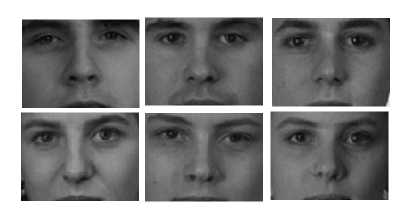
\includegraphics[width=\linewidth]{white.png}}
			
			\column{.50\linewidth}
			\textbf{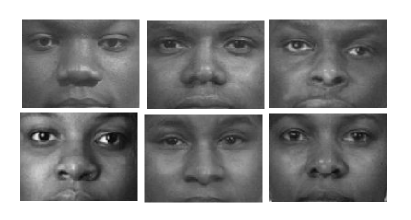
\includegraphics[width=\linewidth]{black.png}}
		\end{columns}
		
		\vspace{1.2mm}
		
		\flushleft 16 Attributes (\textcolor{magenta}{Good, laughter, pleasure, glory, peace, happy, joy, love and} and \textcolor{springgreen}{Evil, bad, horrible, terrible, nasty, pain, failure, hate})
		
	
	\vspace{1.2mm}
	Participants: 62 (F $=48.39$\%, Age = $24.92\pm2.11$ years)
	
	\vspace{1.2mm}
	\textbf{Conditions:}
	\vspace{1.2mm}
	
	WGBB: White-Good/Black-Bad, 60 trials
	
	BGWB: Black-Good/White-Bad, 60 trials
	
\end{frame}



\begin{frame}{Model comparison}
	\begin{spacing}\Factor
		\begin{footnotesize}
			\begin{table}
				\centering
				\begin{tabular}{l l l l l l l l}
					\toprule
					&\multicolumn{3}{c}{Accuracy}
					& & 
					\multicolumn{3}{c}{Response times}\\ 
					\cline{2-4} \cline{6-8}
					Model & AIC & BIC & Deviance& & AIC & BIC & Deviance\\
					\midrule
					1 & $3785.87$ & $3813.53$ & $3777.87$ && $4762.63$ & $4797.2$ & $4752.63$\\
					\textcolor<2->{rasch}{2} & \textcolor<2->{rasch}{$3784.43$} & \textcolor<2->{rasch}{$3825.91$} &  \textcolor<2->{rasch}{$3772.43$} &&  \multicolumn{3}{c}{Aberrant estimates} \\
					
					\textcolor<3->{log}{3} & $3786.51$ & $3828.00$ & $3774.51$ && \textcolor<3->{log}{$4399.66$} & \textcolor<3->{log}{$4448.06$} & \textcolor<3->{log}{$4385.66$}\\
					\bottomrule
				\end{tabular}
			\end{table}
		\end{footnotesize}
		
	\end{spacing}
	\vspace{1.5mm}
	\begin{columns}[T]
		\onslide<2->
		\begin{column}{.5\linewidth}
			{\centering{\color{rasch}{Rasch model:}} \\ \small{Model 2} \\}
			\centering
			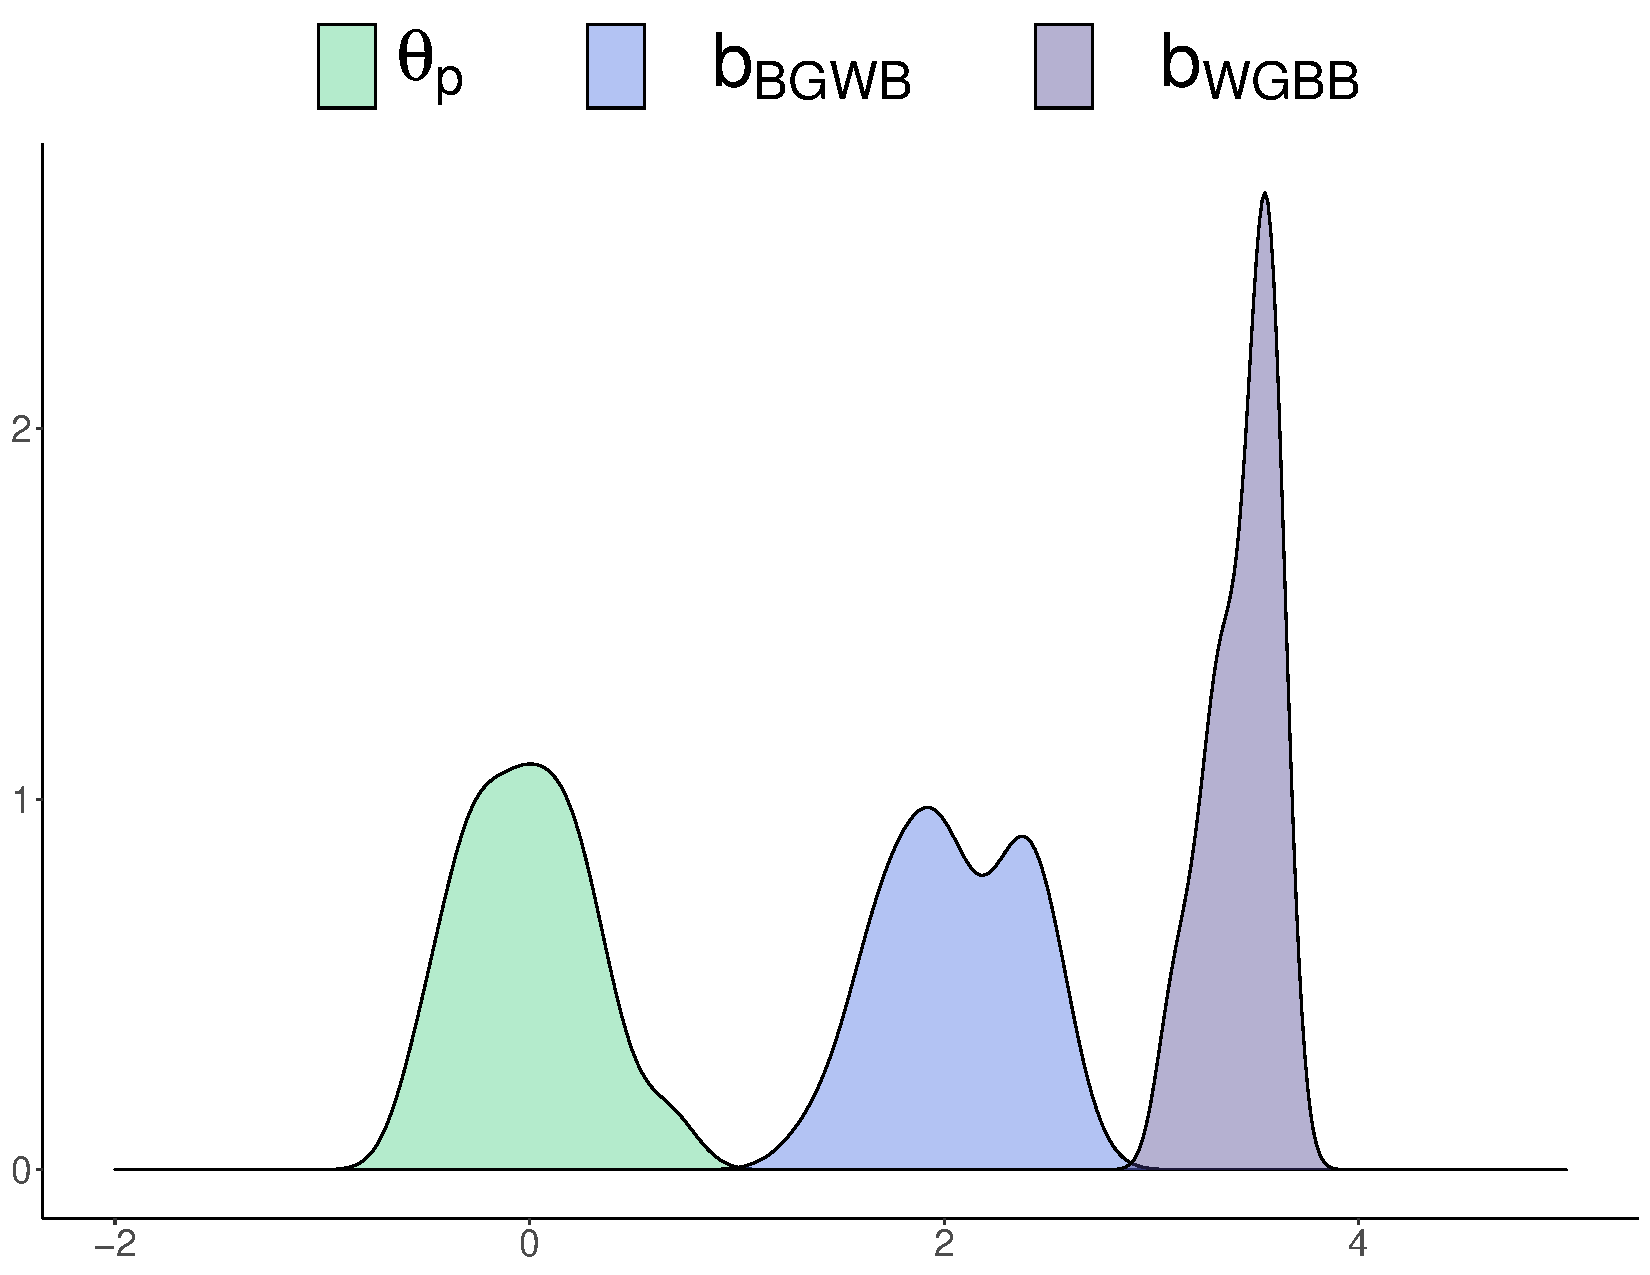
\includegraphics[width=0.8\linewidth]{raceParaccuracy.pdf}
			
		\end{column}
		\onslide<3->
		\begin{column}{.5\linewidth}
			{\centering{\color{log}{Log-normal model:}} \\ \small{Model 3} \\}
			
			\centering
			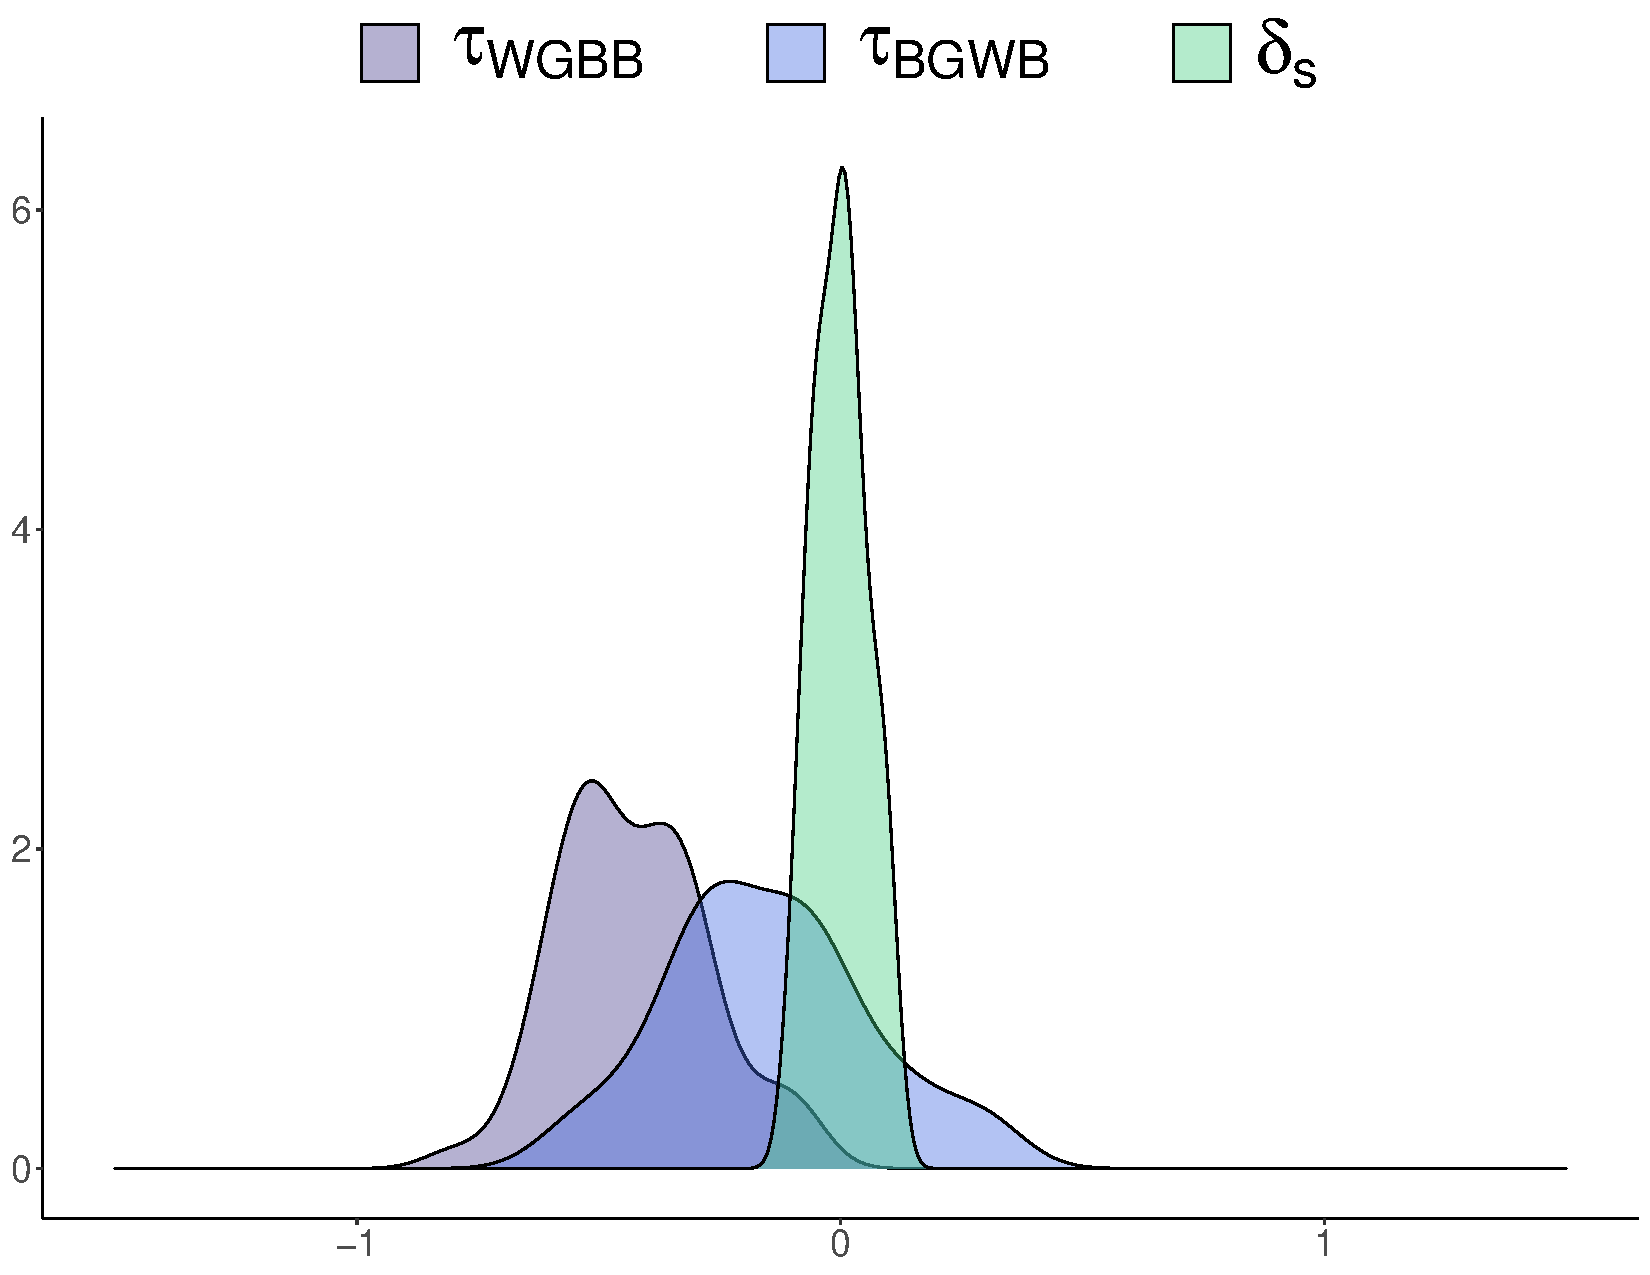
\includegraphics[width=0.8\linewidth]{racePartime.pdf}
			
		\end{column}	
	\end{columns}
\end{frame}



\begin{frame}{Condition--specific easiness}
	
	\vspace{7mm}
	\begin{columns}
		
		\column{.55\linewidth}
		\centering{\textcolor{comp}{\textsc{High contribution stimuli}}}
		
		\vspace{5mm}
		\onslide<1->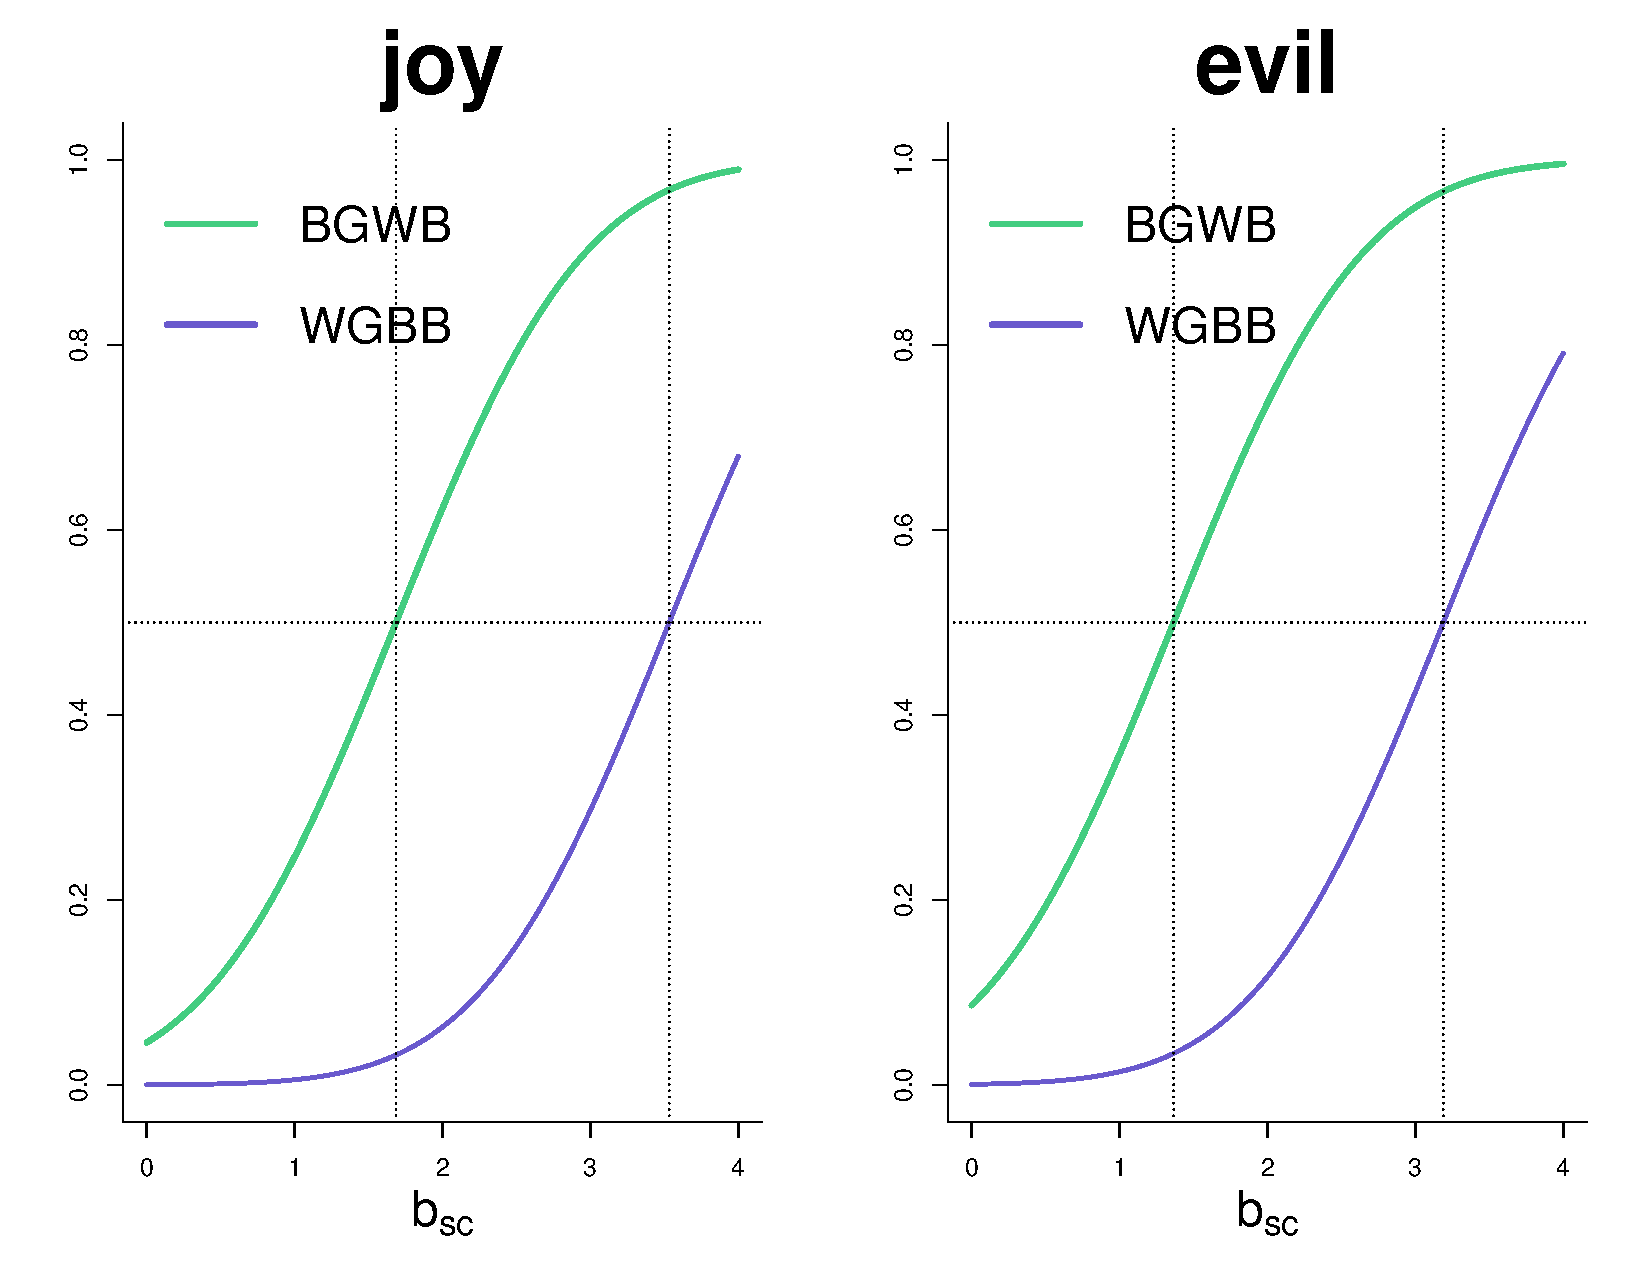
\includegraphics[width=\textwidth]{RaceHigh.pdf}
		
		\column{.55\linewidth}
		\centering{\textcolor{inc}{\textsc{Low contribution stimuli}}}
		
		\vspace{5mm}
		\onslide<1->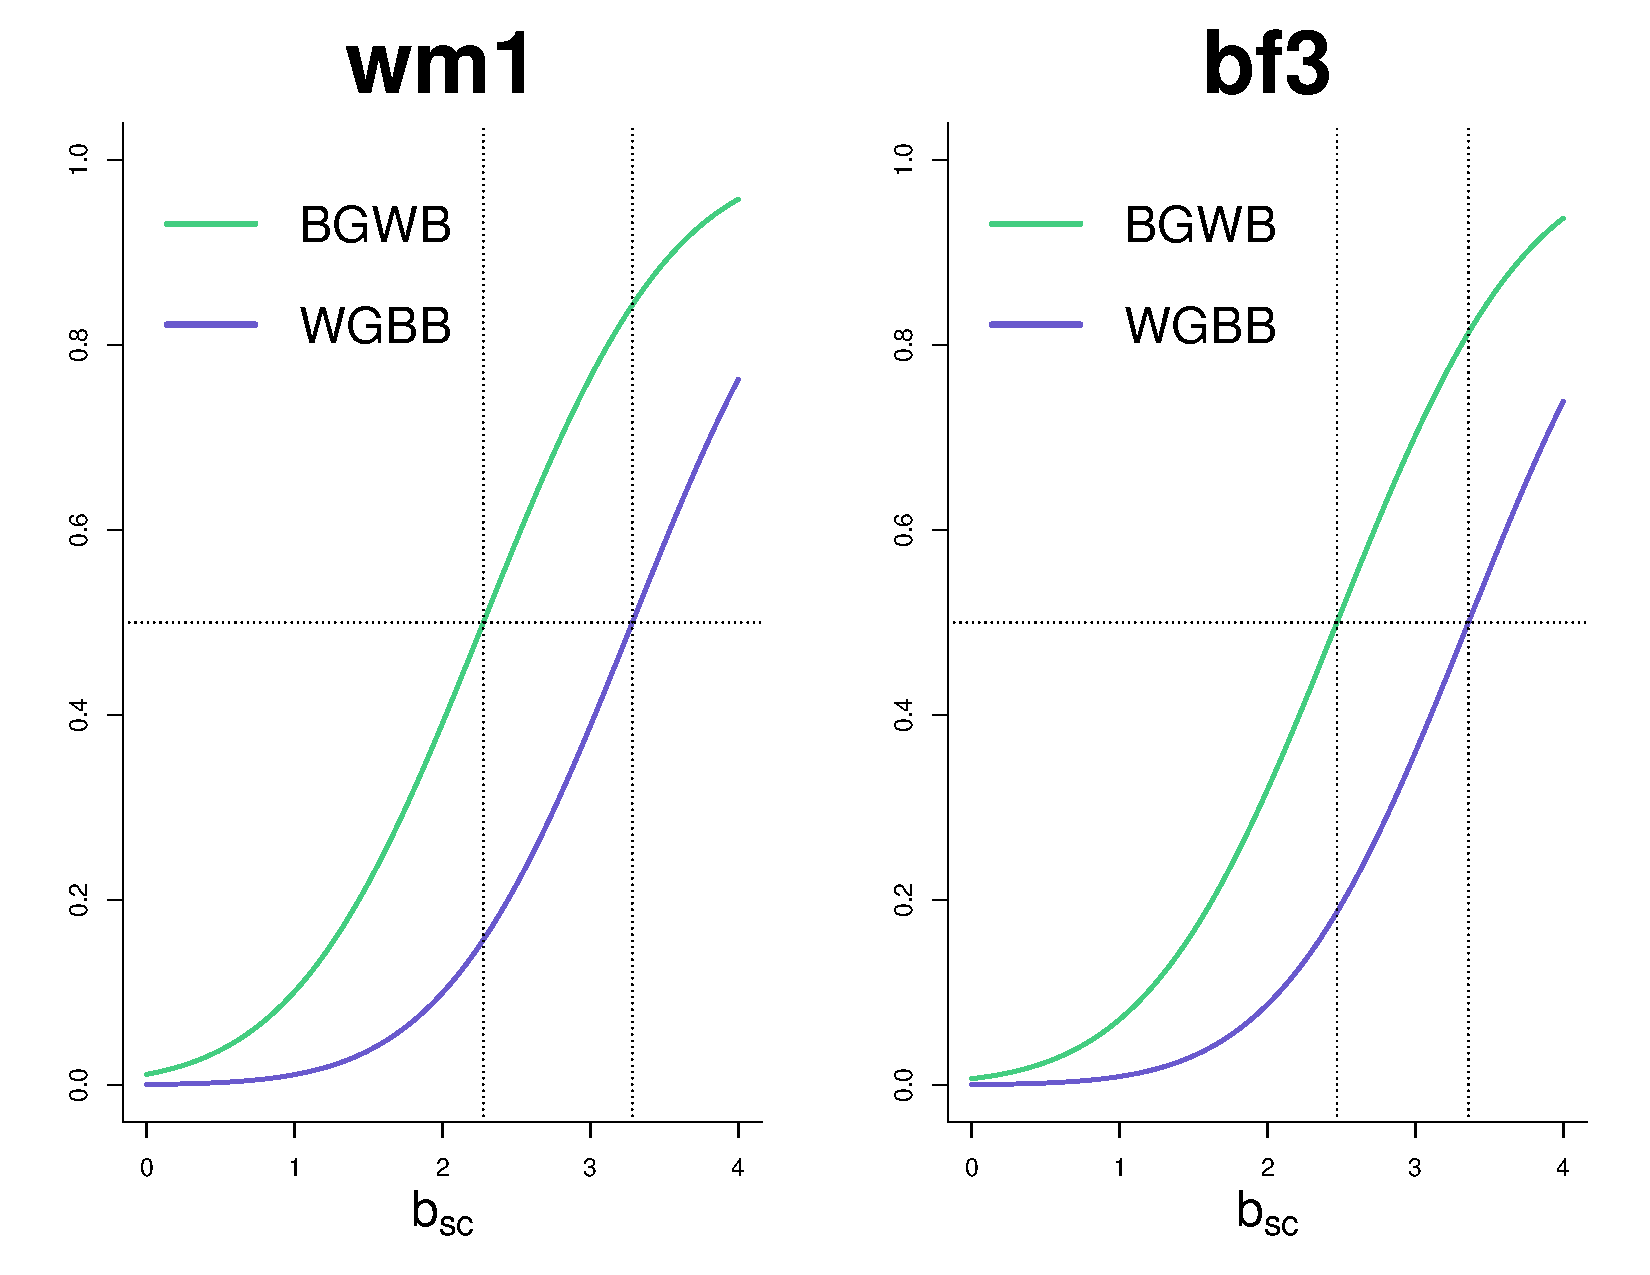
\includegraphics[width=\textwidth]{RaceLow.pdf}
	\end{columns}
	\tikzoverlay (n1) at (7.3cm, 5.3cm){%
		\begin{minipage}{0.1\linewidth}
			\centering	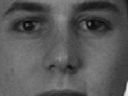
\includegraphics[width=0.68\linewidth]{wm1.jpg}
		\end{minipage}
	}; %
	\tikzoverlay (n2) at (10.3cm, 5.3cm){%
		\begin{minipage}{0.1\linewidth}
			\centering	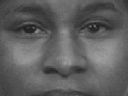
\includegraphics[width=0.68\linewidth]{bf56.jpg}
		\end{minipage}
	}; %
	%\vspace{\fill}
\end{frame}

%\subsection*{Stimuli time intensity}
\begin{frame}{Overall time intensity}
	\begin{columns}[T]
		\begin{column}{.5\linewidth}
			\centering \emph{\textcolor{springgreen}{Bad}} \& \textcolor{magenta}{\emph{Good}}
			\vspace{5mm}
			\begin{figure}
				\centering
				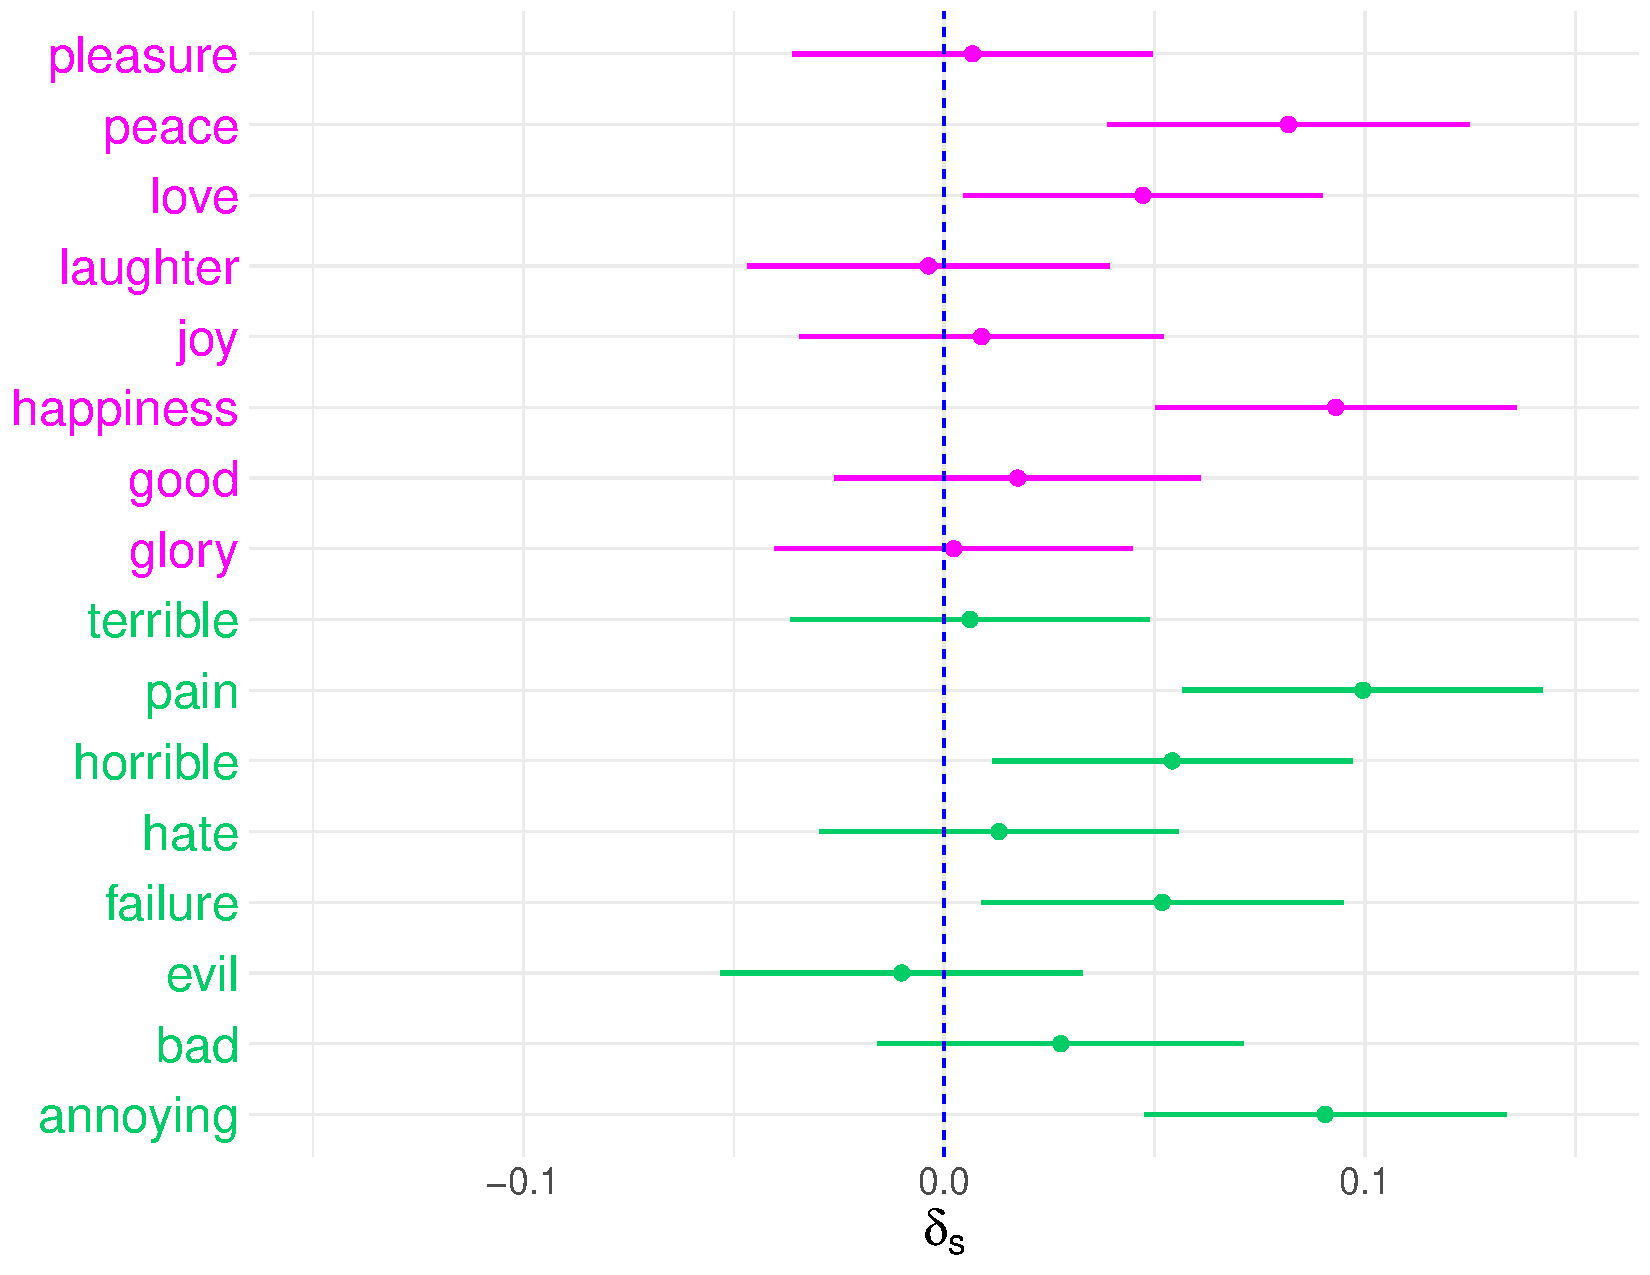
\includegraphics[width=\linewidth]{raceIntensityWords.pdf}				
			\end{figure}
			
		\end{column}
		
		\begin{column}{.5\linewidth}
			\centering \emph{\textcolor{royalblue3}{Black}} \& \emph{\textcolor{orangered2}{White}}
			\vspace{5mm}
			\begin{figure}
				\centering
				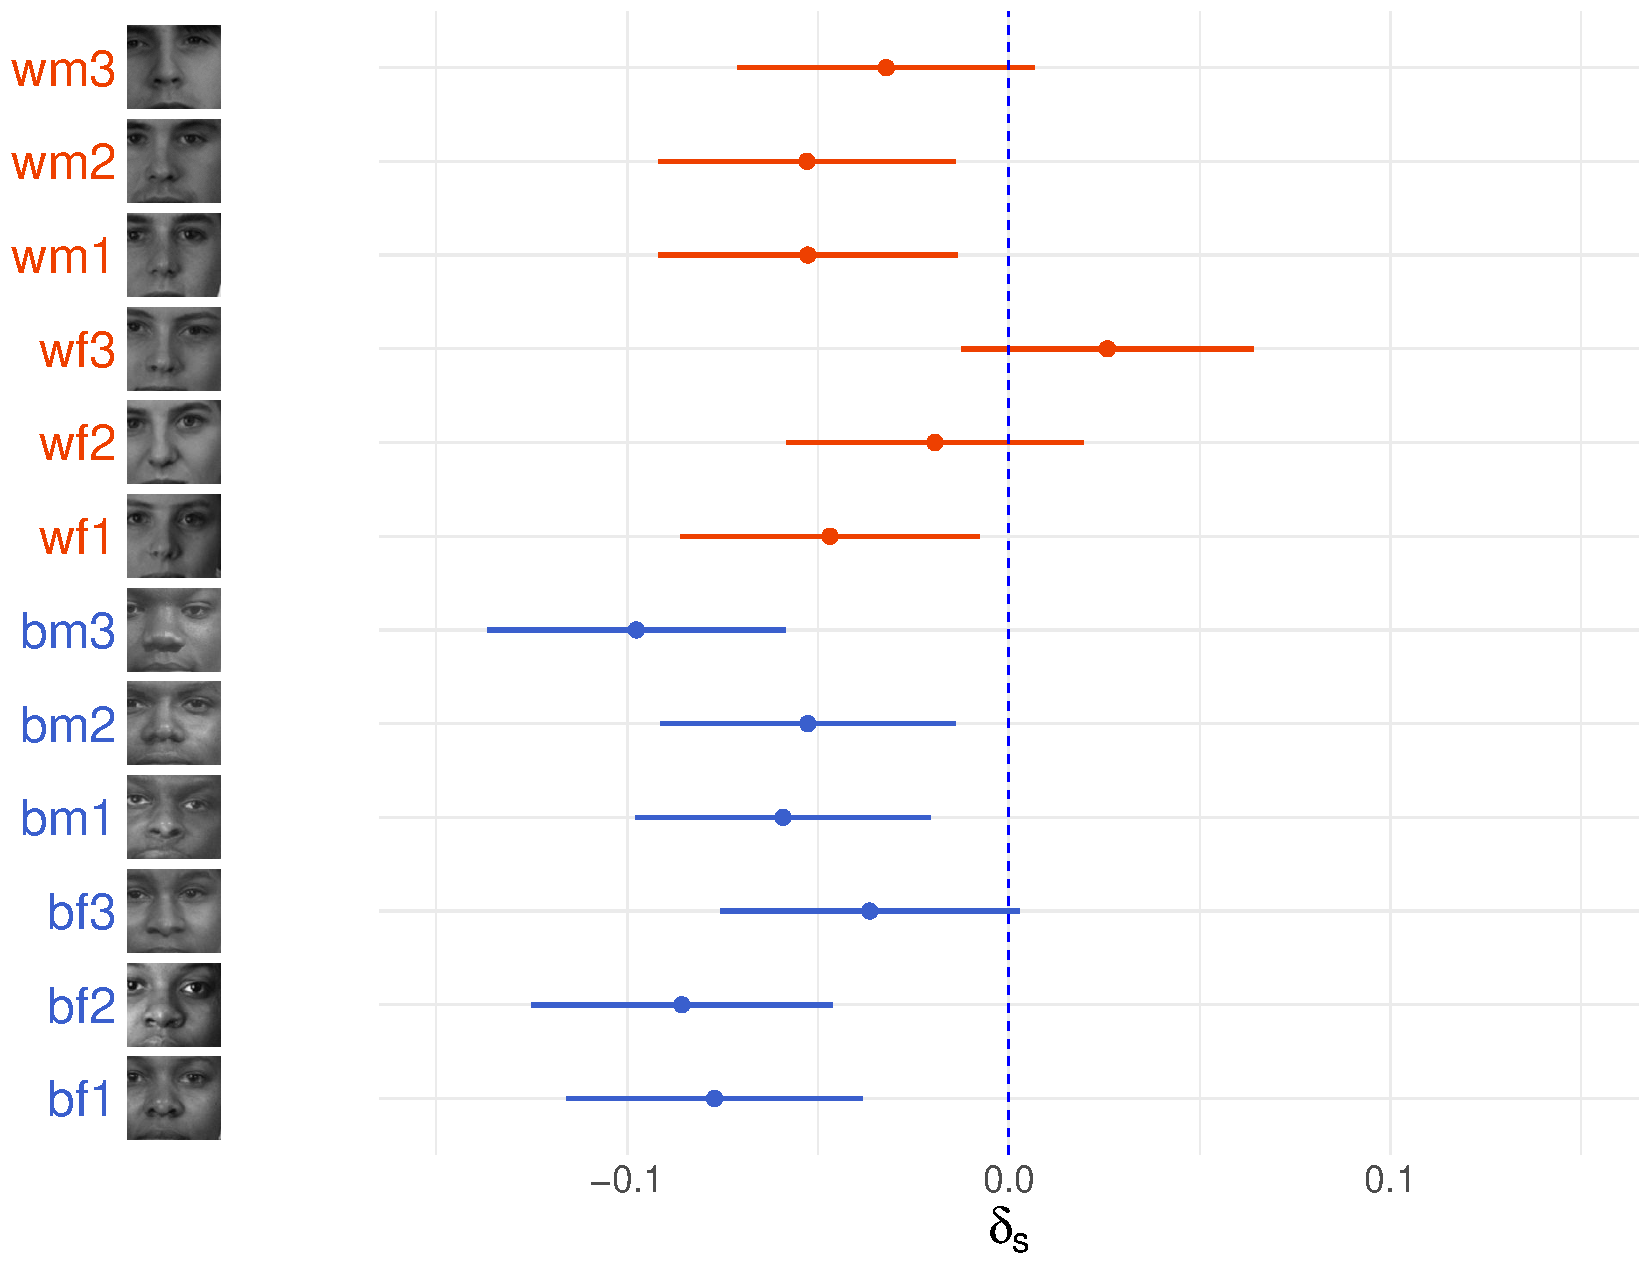
\includegraphics[width=\linewidth]{raceIntensityPics.pdf}
			\end{figure}
			
		\end{column}	
	\end{columns}
\end{frame}

\section[Make it easy]{The easy way}

\begin{frame}
	%	\begin{spacing}\Factor
	\begin{table}[th!]
		\centering
		\begin{tabular}{llll}
			\hline
			\emph{D-score} & Error inflation & Delete trials $<$ 400 ms\\\hline
			\emph{D}1 & Built-in correction & No \\
			\emph{D}2 & Built-in correction & Yes \\
			\emph{D}3 & \emph{M} (correct responses) + 2\emph{sd} & No\\
			\emph{D}4 & \emph{M} (correct responses) + 600 ms & No \\
			\emph{D}5 & \emph{M} (correct responses) + 2\emph{sd} & Yes\\
			\emph{D}6 & \emph{M} (correct responses) + 600 ms & Yes \\\hline
		\end{tabular}
	
	\end{table}
	\begin{itemize}
		\item[\large{\Sadey}] Few Open source alternatives
		\item[\large{\Sadey}] Utterly complicated to use
		\item[\large{\Sadey}] No clear information on the algorithm they compute
		\item[\large{\Sadey}] No graphical representation of the results
	\end{itemize}
	
	\vspace{3mm}
	\pause
	\begin{tabular}{l p{9cm}}
		{
\includegraphics[height=5ex]{emoji.png}} & Something Open Source, able to compute multiple scores, and to provide nice graphical representations\\
	\end{tabular}

\end{frame}

\begin{frame}{Make it easy \& Clear}
	\href{https://cran.r-project.org/web/packages/implicitMeasures/index.html}{\texttt{implicitMeasures} package} DOI:\href{https://joss.theoj.org/papers/10.21105/joss.02394}{10.21105/joss.02394} : 
	
	\vspace{2mm}
	\begin{small}
		\begin{tabular}{p{2.3cm}p{8cm}}
			\hline
			Function & Description \\
			\hline
			\texttt{clean\_iat()} & Prepare and clean IAT data\\
			\texttt{clean\_sciat()} & Prepare and clean SC-IAT data\\
			\texttt{compute\_iat()} & Compute IAT \emph{D-score}\\
			\texttt{compute\_sciat()} & Compute SC-IAT \emph{D-score} \\
			\texttt{descript\_d()} & Descriptive table of \emph{D-score}s (even in \LaTeX) \\  
			\texttt{d\_density()} & Plot IAT or SC-IAT scores (distribution)\\
			\texttt{d\_point()} & Plot either IAT or SC-IAT scores (points)\\
			\texttt{IAT\_rel()} & IAT reliability\\
			\texttt{multi\_dsciat()} & Plot SC-IATs scores\\
			\texttt{multi\_dscore()} & Compute and plot multiple \emph{D-score}s\\
			\texttt{raw\_data()} & Dataset with one IAT and two SC-IATs\\
			\hline
		\end{tabular}
	\end{small}
	
	\begin{small}
		\begin{itemize}
			\item \href{https://cran.r-project.org/web/packages/implicitMeasures/vignettes/implicitMeasures.html}{\textcolor{blue}{implicitMeasures}}: Introduction to IAT, SC-IAT, and \emph{D score}s.
			\item \href{https://cran.r-project.org/web/packages/implicitMeasures/vignettes/IAT-example.html}{\textcolor{blue}{IAT-example}}: Package illustration on IAT data
			\item \href{https://cran.r-project.org/web/packages/implicitMeasures/vignettes/SC-IAT-example.html}{\textcolor{blue}{SC-IAT-example}}: Package illustration on SC-IAT data
		\end{itemize}
	\end{small}
\end{frame}

\begin{frame}{Make it even easier}
	\begin{center}
		\href{http://fisppa.psy.unipd.it/DscoreApp/}{
\includegraphics[width=0.4\linewidth]{AppLogo.png}}
	\end{center}
	\vspace{5mm}
	\color{black}
	Source code on \href{https://github.com/OttaviaE/DscoreApp}{\textcolor{blue}{GitHub}}	
	
	\vspace{3mm}
	DOI: \href{https://www.frontiersin.org/articles/10.3389/fpsyg.2019.02938/full}{10.3389/fpsyg.2019.02938}
\end{frame}

\section*{Thanks}
\begin{frame}
	\centering

	Thank you!
	
		\vspace{5mm}
	
	\texttt{ottavia.epifania@unipd.it}
\end{frame}

\end{document}
